\section{Detector infrastructure}
\label{ch:dp-tc-infrastructure}

ACCESS TO THE ROOF

The detector infrastructure for the \dword{dpmod} comprises the equipment used by several groups to install and operate the detector.
It includes the electronics racks on top of the mezzanine on the cryostat roof and the related networking, electrical and cooling power, cable trays, cryostat penetrations and flanges, detector ground isolation transformers and monitors.
Inside the cryostat, the detector infrastructure includes the gas and liquid argon distribution manifolds, the cryostat false floor to protect the corrugated membrane and allow safe circulation of material and people inside the cryostat, movable scaffolding and man lifts for activities at height.
A clean room equipped with cold boxes for the functional tests of the \dwords{crp} is also present in front of the \dword{tco}.
This clean room and the cryostat itself are the places where some detector components are assembled before installation.

\subsection{Cryostat roof}
A drawing of the full cryostat roof with its penetrations is shown in figure~\ref{fig:DP-roof-penetration}.
A zoom of the same image of a corner on the opposite side of the \dword{tco} is shown in figure~\ref{fig:DP-roof-penetration-zoom}.
The same figure shows also the \threed model of the roof with equipment on the \dword{crp} support and \dword{sgft} penetrations. \fixme{what is sgft?}
This image highlights the high density of the equipment on the \dword{dpmod} roof, even more important considering that each of these flanges will be reached by several cables.

\begin{dunefigure}[Drawing of \dword{dpmod} roof]{fig:DP-roof-penetration}
{Drawing of the cryostat roof with its penetration.}
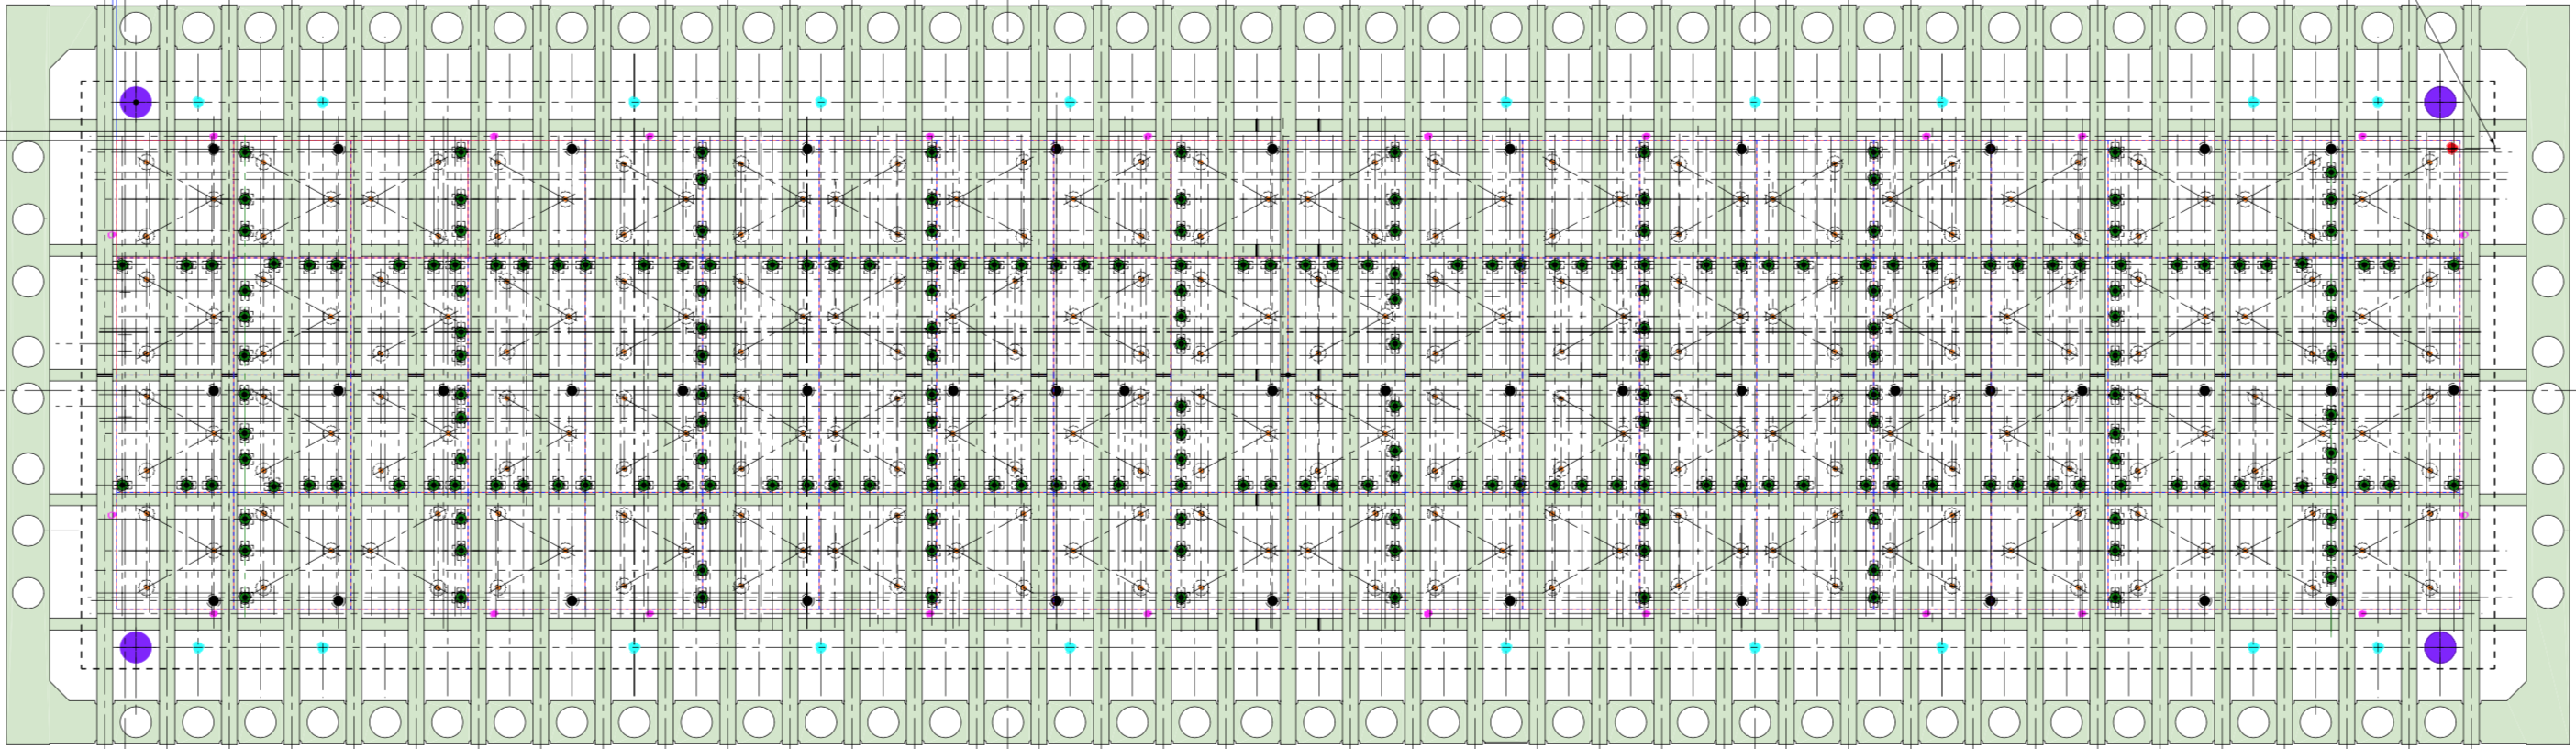
\includegraphics[width=1.\textwidth]{DP-roof-penetration.png}
\end{dunefigure}

\begin{dunefigure}[Zoom of the \dword{dpmod} roof]{fig:DP-roof-penetration-zoom}
{Zoom of the \dword{dpmod} roof drawing (left) and 3D model of the same portion of the roof with the \dword{sgft} and \dword{crp} suspension chimneys instrumented.}
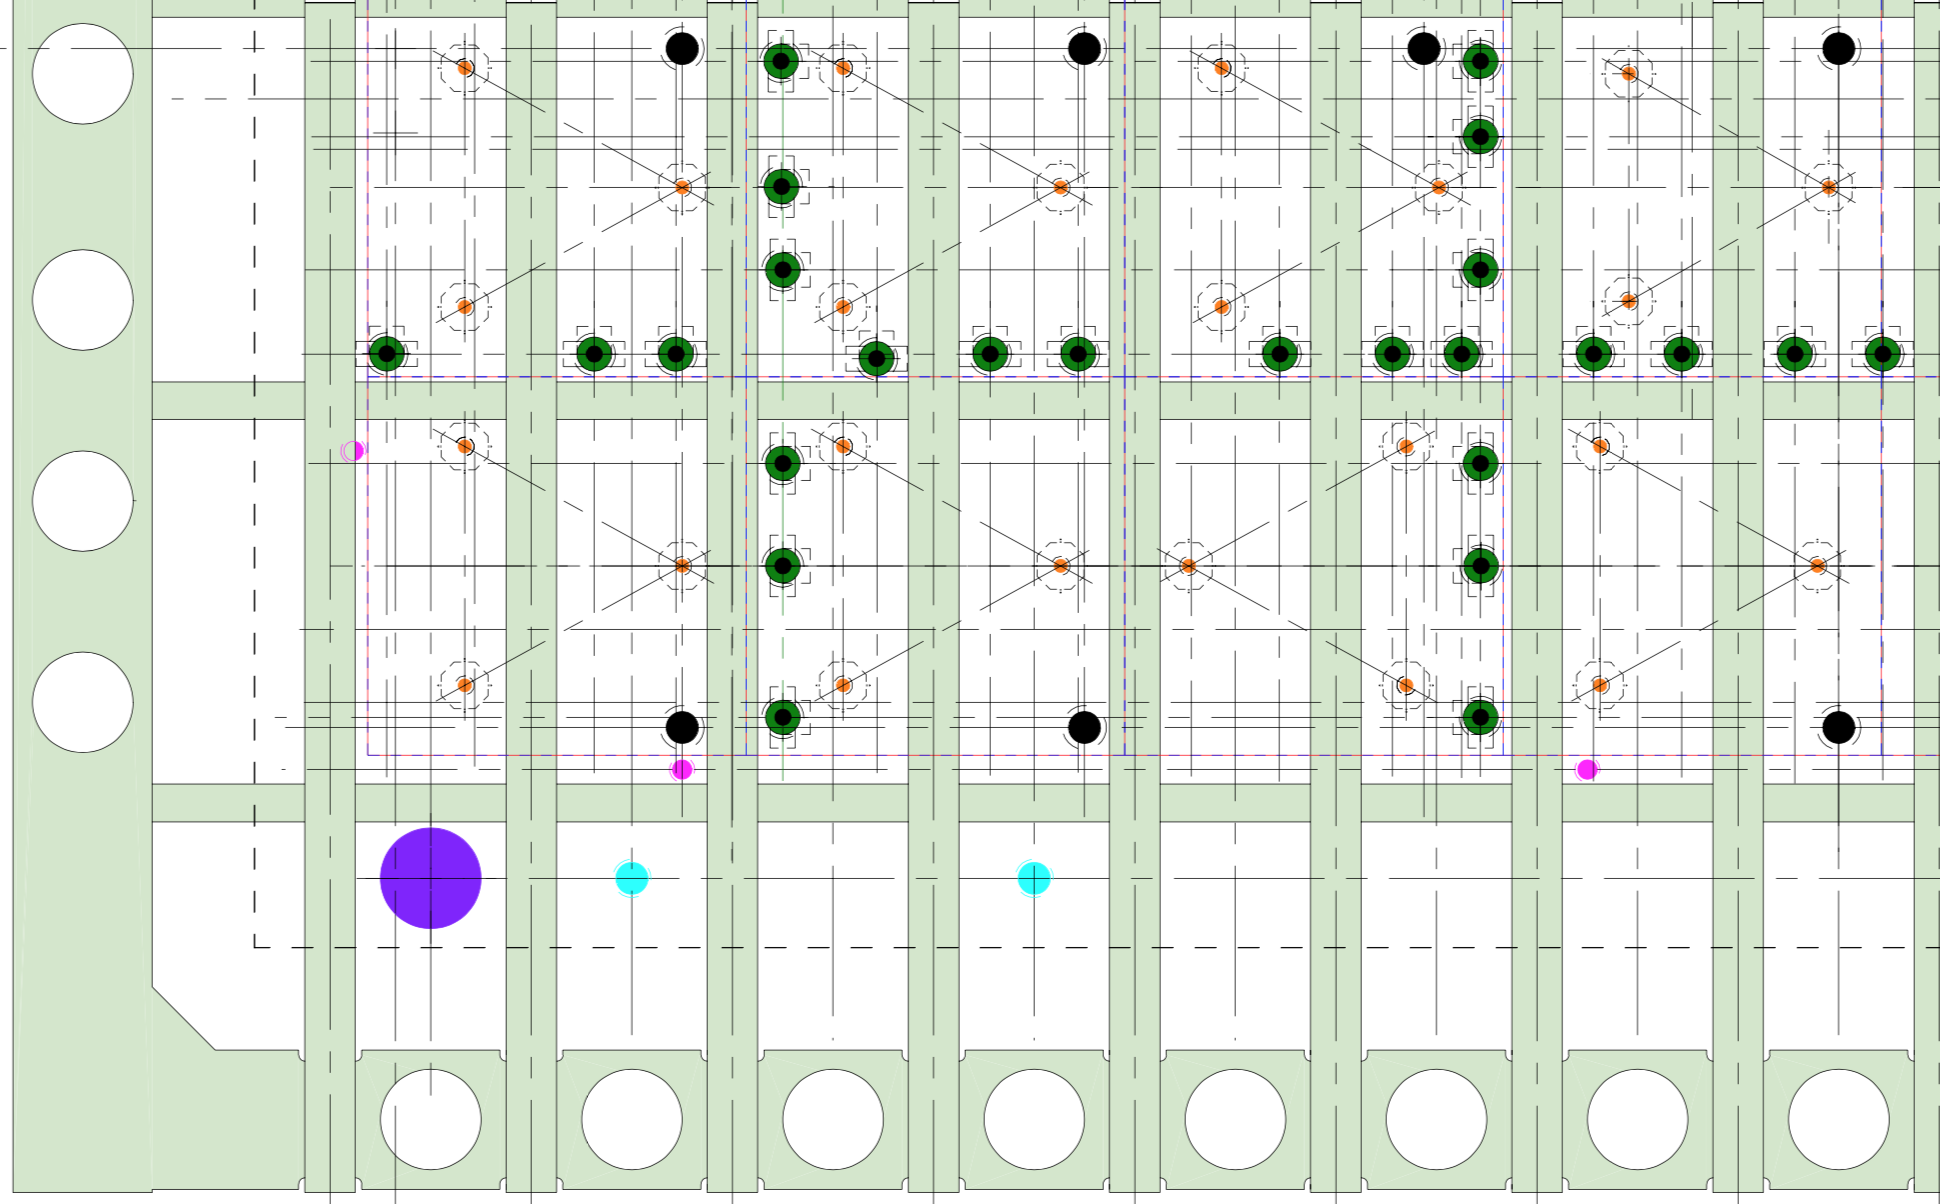
\includegraphics[width=0.5\textwidth]{DP-roof-penetration-zoom.png}
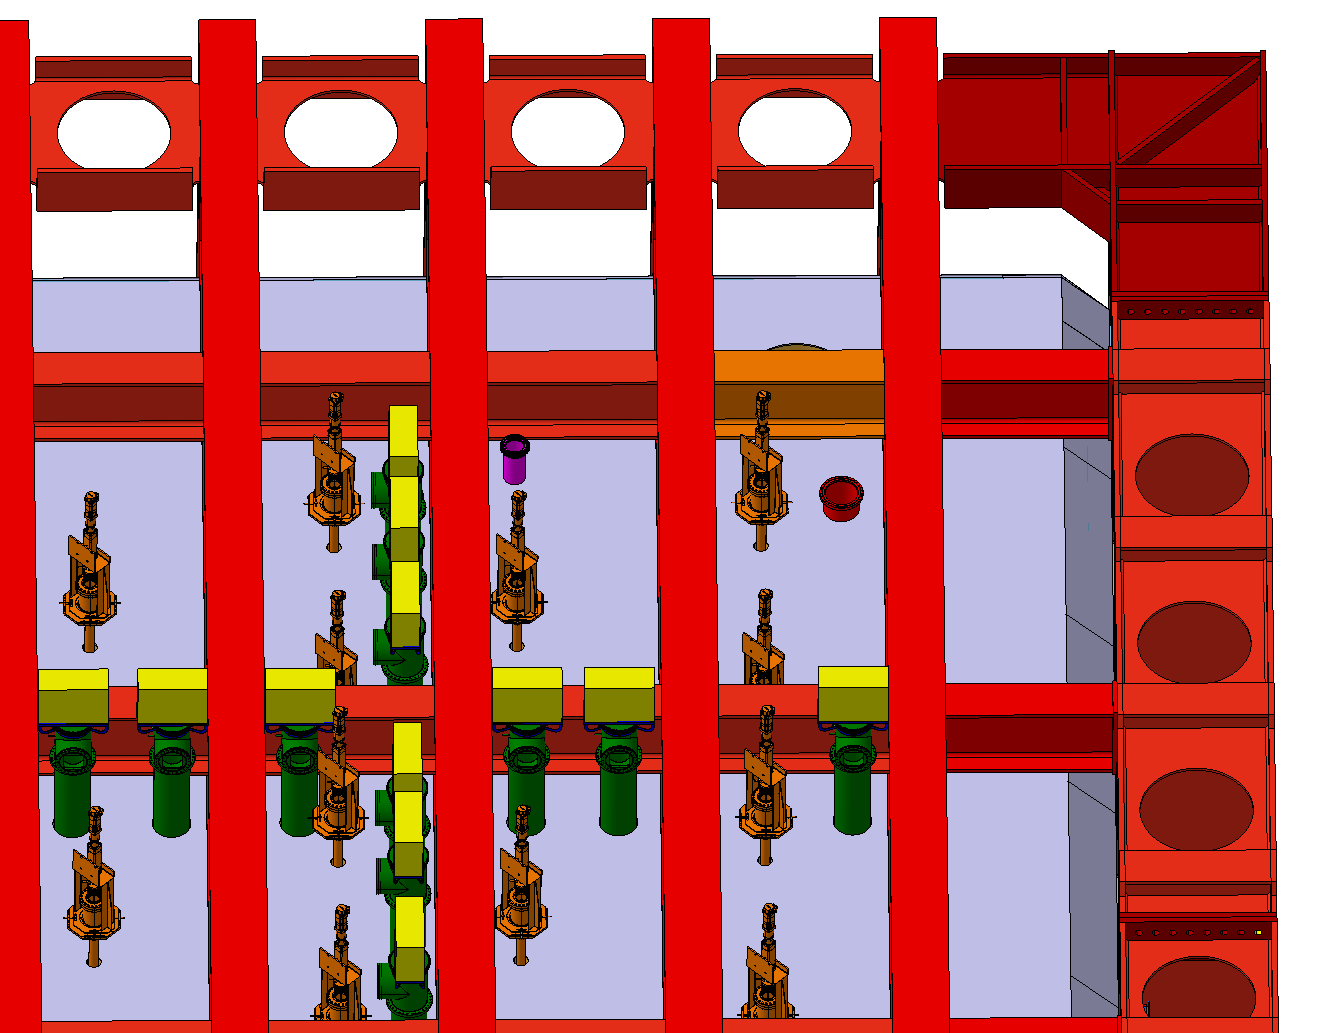
\includegraphics[width=0.5\textwidth]{DP-roof-penetration-3D.png}
\end{dunefigure}

The role of the penetrations is to \emph{connect} the ultra-pure argon volume to the atmosphere through the roof insulation, while minimising the heat input.
All the penetrations are on the roof of the cryostat except the ones for the liquid argon re-circulation that are at the bottom of the \dword{tco} wall.
The sketch of a typical roof penetration cross-section is shown in figure~\ref{fig:penetration-cross-section-sketch}.
\begin{dunefigure}[Sketch of a typical roof penetration]{fig:penetration-cross-section-sketch}
{Sketch of a typical roof penetration.}
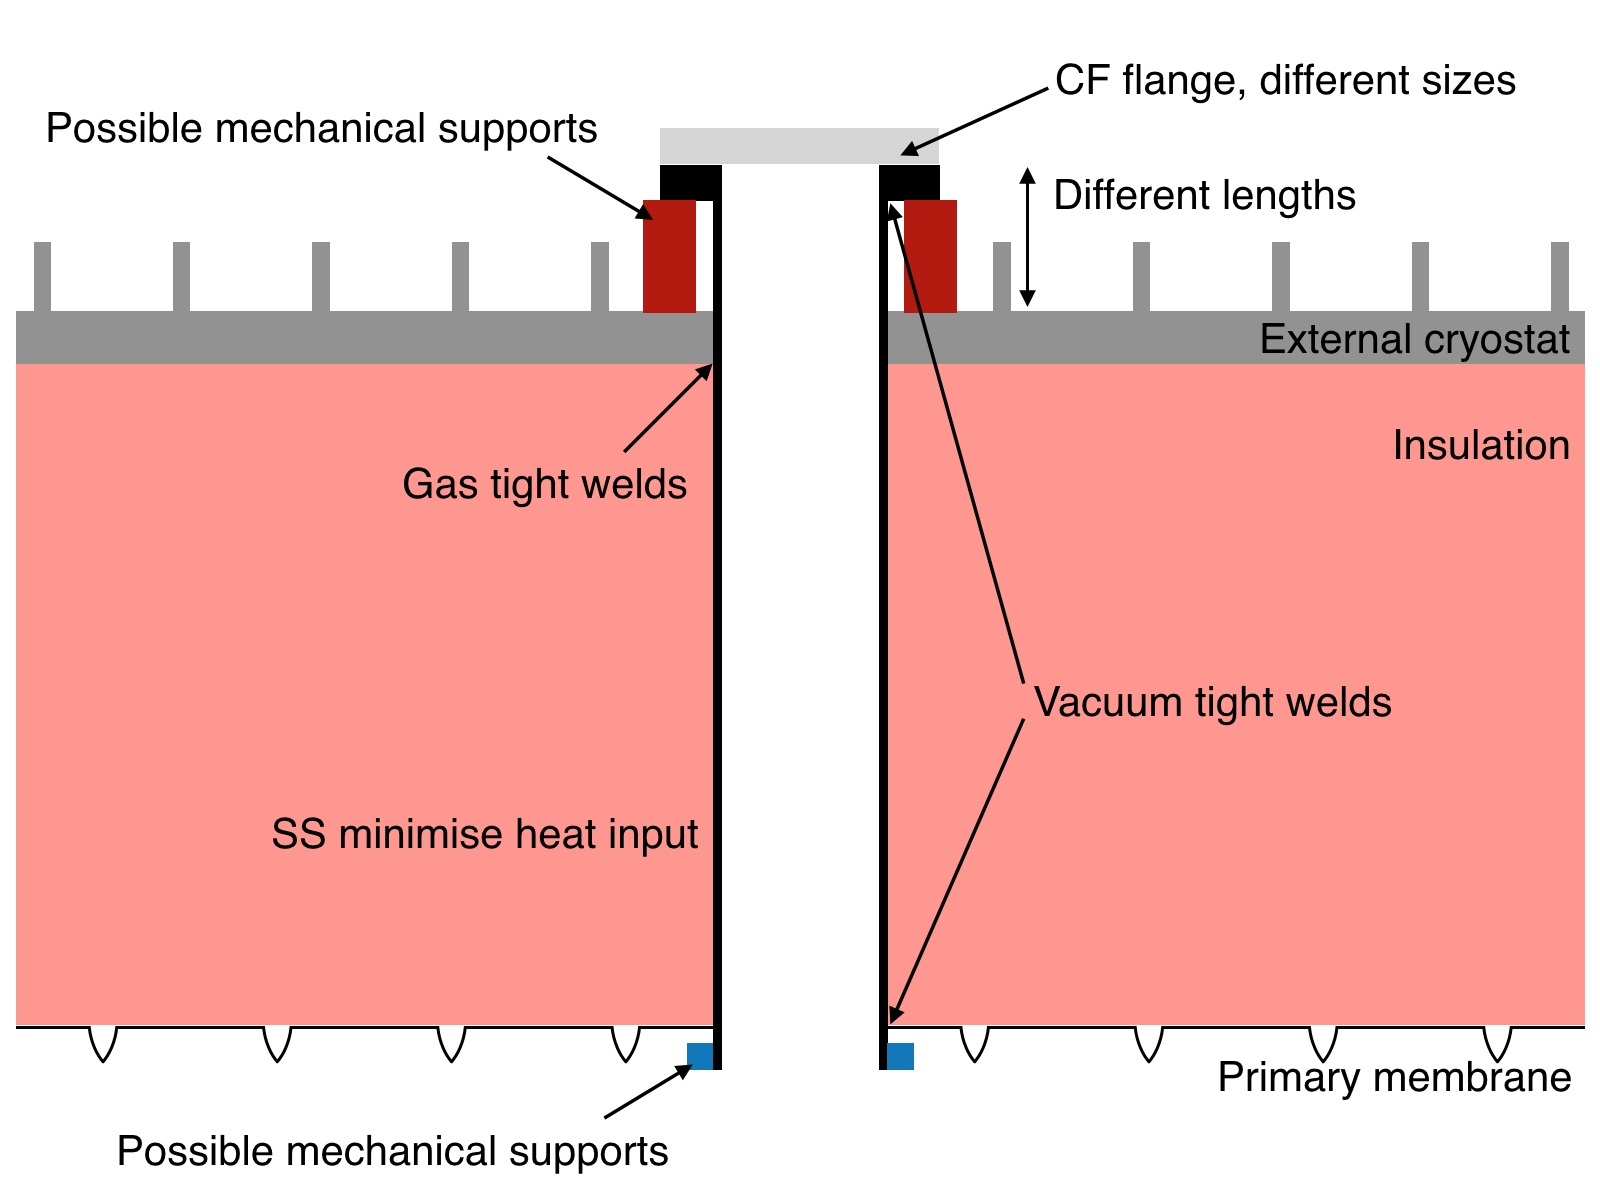
\includegraphics[width=1.\textwidth]{penetration-cross-section-sketch.png}
\end{dunefigure}
The thermal insulation is installed around a vertical stainless steel pipe that is mechanically connected to the walls of the warm structure.
The corrugated membrane is welded vacuum tight to the pipes.
The excess pipe inside the cryostat volume may be used to weld a mechanical support, for instance to attach cable trays.
On the atmospheric side a \dword{uhv} CF flange is welded vacuum tight to the pipe. \fixme{Define UHV in glossary}
Except for the four man holes, all the flanges on the chimneys follow the \dword{uhv} CF flange standard ISO 3669:2017.
These flanges may need to be supported in case they must sustain some load, as for example in the case of the penetrations for the \dword{crp} and field cage supports.
These flanges carry out the role of interface between the cryostat and the feedthroughs.
The scope of the detector infrastructure ends at the flange.
Copper gaskets, bolts, and nuts are in the scope of the mating flange.
The holes on the cryostat flanges are not threaded.
In order to allow an effective air purge, each feedthrough must foresee an exhaust positioned preferably at the maximum hight in order to avoid air pockets.
For reasons of space, the purge lines for the \dword{sgft} are embedded in the stainless steel pipe of the penetrations.
COMMENT ON THE VALVES

CONSTRAINTS ON THE LINEARITY OF THE PIPE, ON THE VERTICALITY OF THE PIPE AND ON THE HORIZONTALITY OF THE FLANGE AND ON THE ORIENTATION OF THE FLANGE.
REQUIREMENT ON THE TIGHTNESS

There are several kinds of penetrations that serves different needs.
The table~\ref{tab:penetrations} summarises the them.
\begin{dunetable}[Types of penetrations through the roof]
{ccccccc}
{tab:penetrations}
{Types of penetrations through the roof.}
Type & Number & CF & Pipe OD (mm) & Pipe ID (mm) & Ext. Sup. & Int. Sup.\\
\toprowrule \dword{crp} sup. & 240 & CF100 & 104 & 100 & yes & no\\
\colhline Field cage sup. & 24 & CF150 & 154 & 150 & yes & no\\
\colhline \dword{crp} inst. & 42 & CF250 & 254 & 250 & no & yes\\
\colhline Tank inst. & 20 & CF250 & 254 & 250 & no & yes\\
\colhline \dword{sgft} & 240 & CF275 & 273.2 & 267 & no & no\\
\colhline VHV & 1 & CF250 & 254 & 250 & no & yes\\
\colhline Manhole & 4 & custom & 706 & 700 & no & no\\
\colhline Cryo & 39 & several & several & several & several & several\\
\end{dunetable}

TABLE WITH THE WEIGHTS THAT THE MECHANICAL FEEDTHROUGHS MUST SUPPORT
\begin{dunetable}[Load for mechanical support penetrations]
{ccccc}
{tab:load-penetration}
{Load for mechanical support penetrations.}
Type & Number & Installation (kg) & Empty (kg) & Full (kg) \\
\toprowrule \dword{crp} sup. & 240 & 150 & 150 & 150\\
\colhline Field cage sup. & 24 & XXX & XXX & XXX \\
\end{dunetable}

BRIEF DESCRIPTION OF THE \dword{crp} SUPPORTS. NOTE THAT THE THERE ARE TWO TYPES OF TRIANCLES. NOTE ALLOW SHRINKAGE AND RE-ADJUSTMENT IN 4X4 CRPS ISLANDS

BRIEF DESCRIPTION OF THE FIELD CAGE SUPPORT. NOTE THAT ON THE SHORT WALLS THE EXTERNAL I-BEAM ARE VERY CLOSE TO THE PENETRATOINS. NOTE ALLOW SHRINKAGE.

BRIEF DESCRIPTION OF THE \dword{crp} INSTRUMENTATION. NOTE THAT THEY SERVE TWO CRPS AND NOT ALSWAYS WAS POSSIBLE TO PUT THEM IN THE RIGHT PLACE. NEED TO DEVELOP AND APPROPRIATE CABLE SUPPORTING SYETEM.

BRIEF DESCRIPTION OF THE TANK INSTRUMENTATION. NOTE THAT NO CABLE TRAYS ARE ALOWED TO BE ATTACHED TO THE CORRUGATED MEMBRANE. DEDICATED CABLE SUPPORTS AND USE THE CRYOGENIC PIPES AS CABLE TRAY WHEREVER POSSIBLE.

BRIEF DESCRIPTION OF THE VHV PENETRATION. NOTE THAT IT IS IN THE ACTIVE VOLUME. THAT CRP IS DIFFERENT.

The \dword{sgft} were developed first for the 3x1x1 detector at \dword{cern} and then applied to the \dword{pddp} with a slightly different design.
Their role is to allow the electronics to be near the anode electrodes (minimise the cable lengths) and in cold (reduce the intrinsic noise of the electronics) while still having the possibility to extract the electronics without compromising the liquid argon purity.
The drawing of the \dword{sgft} used in \dword{pddp} is shown in figure~\ref{fig:sgft-drawing}.
\begin{dunefigure}[\dword{sgft} drawing]{fig:sgft-drawing}
{Drawing of the \dword{sgft} used in \dword{pddp}.}
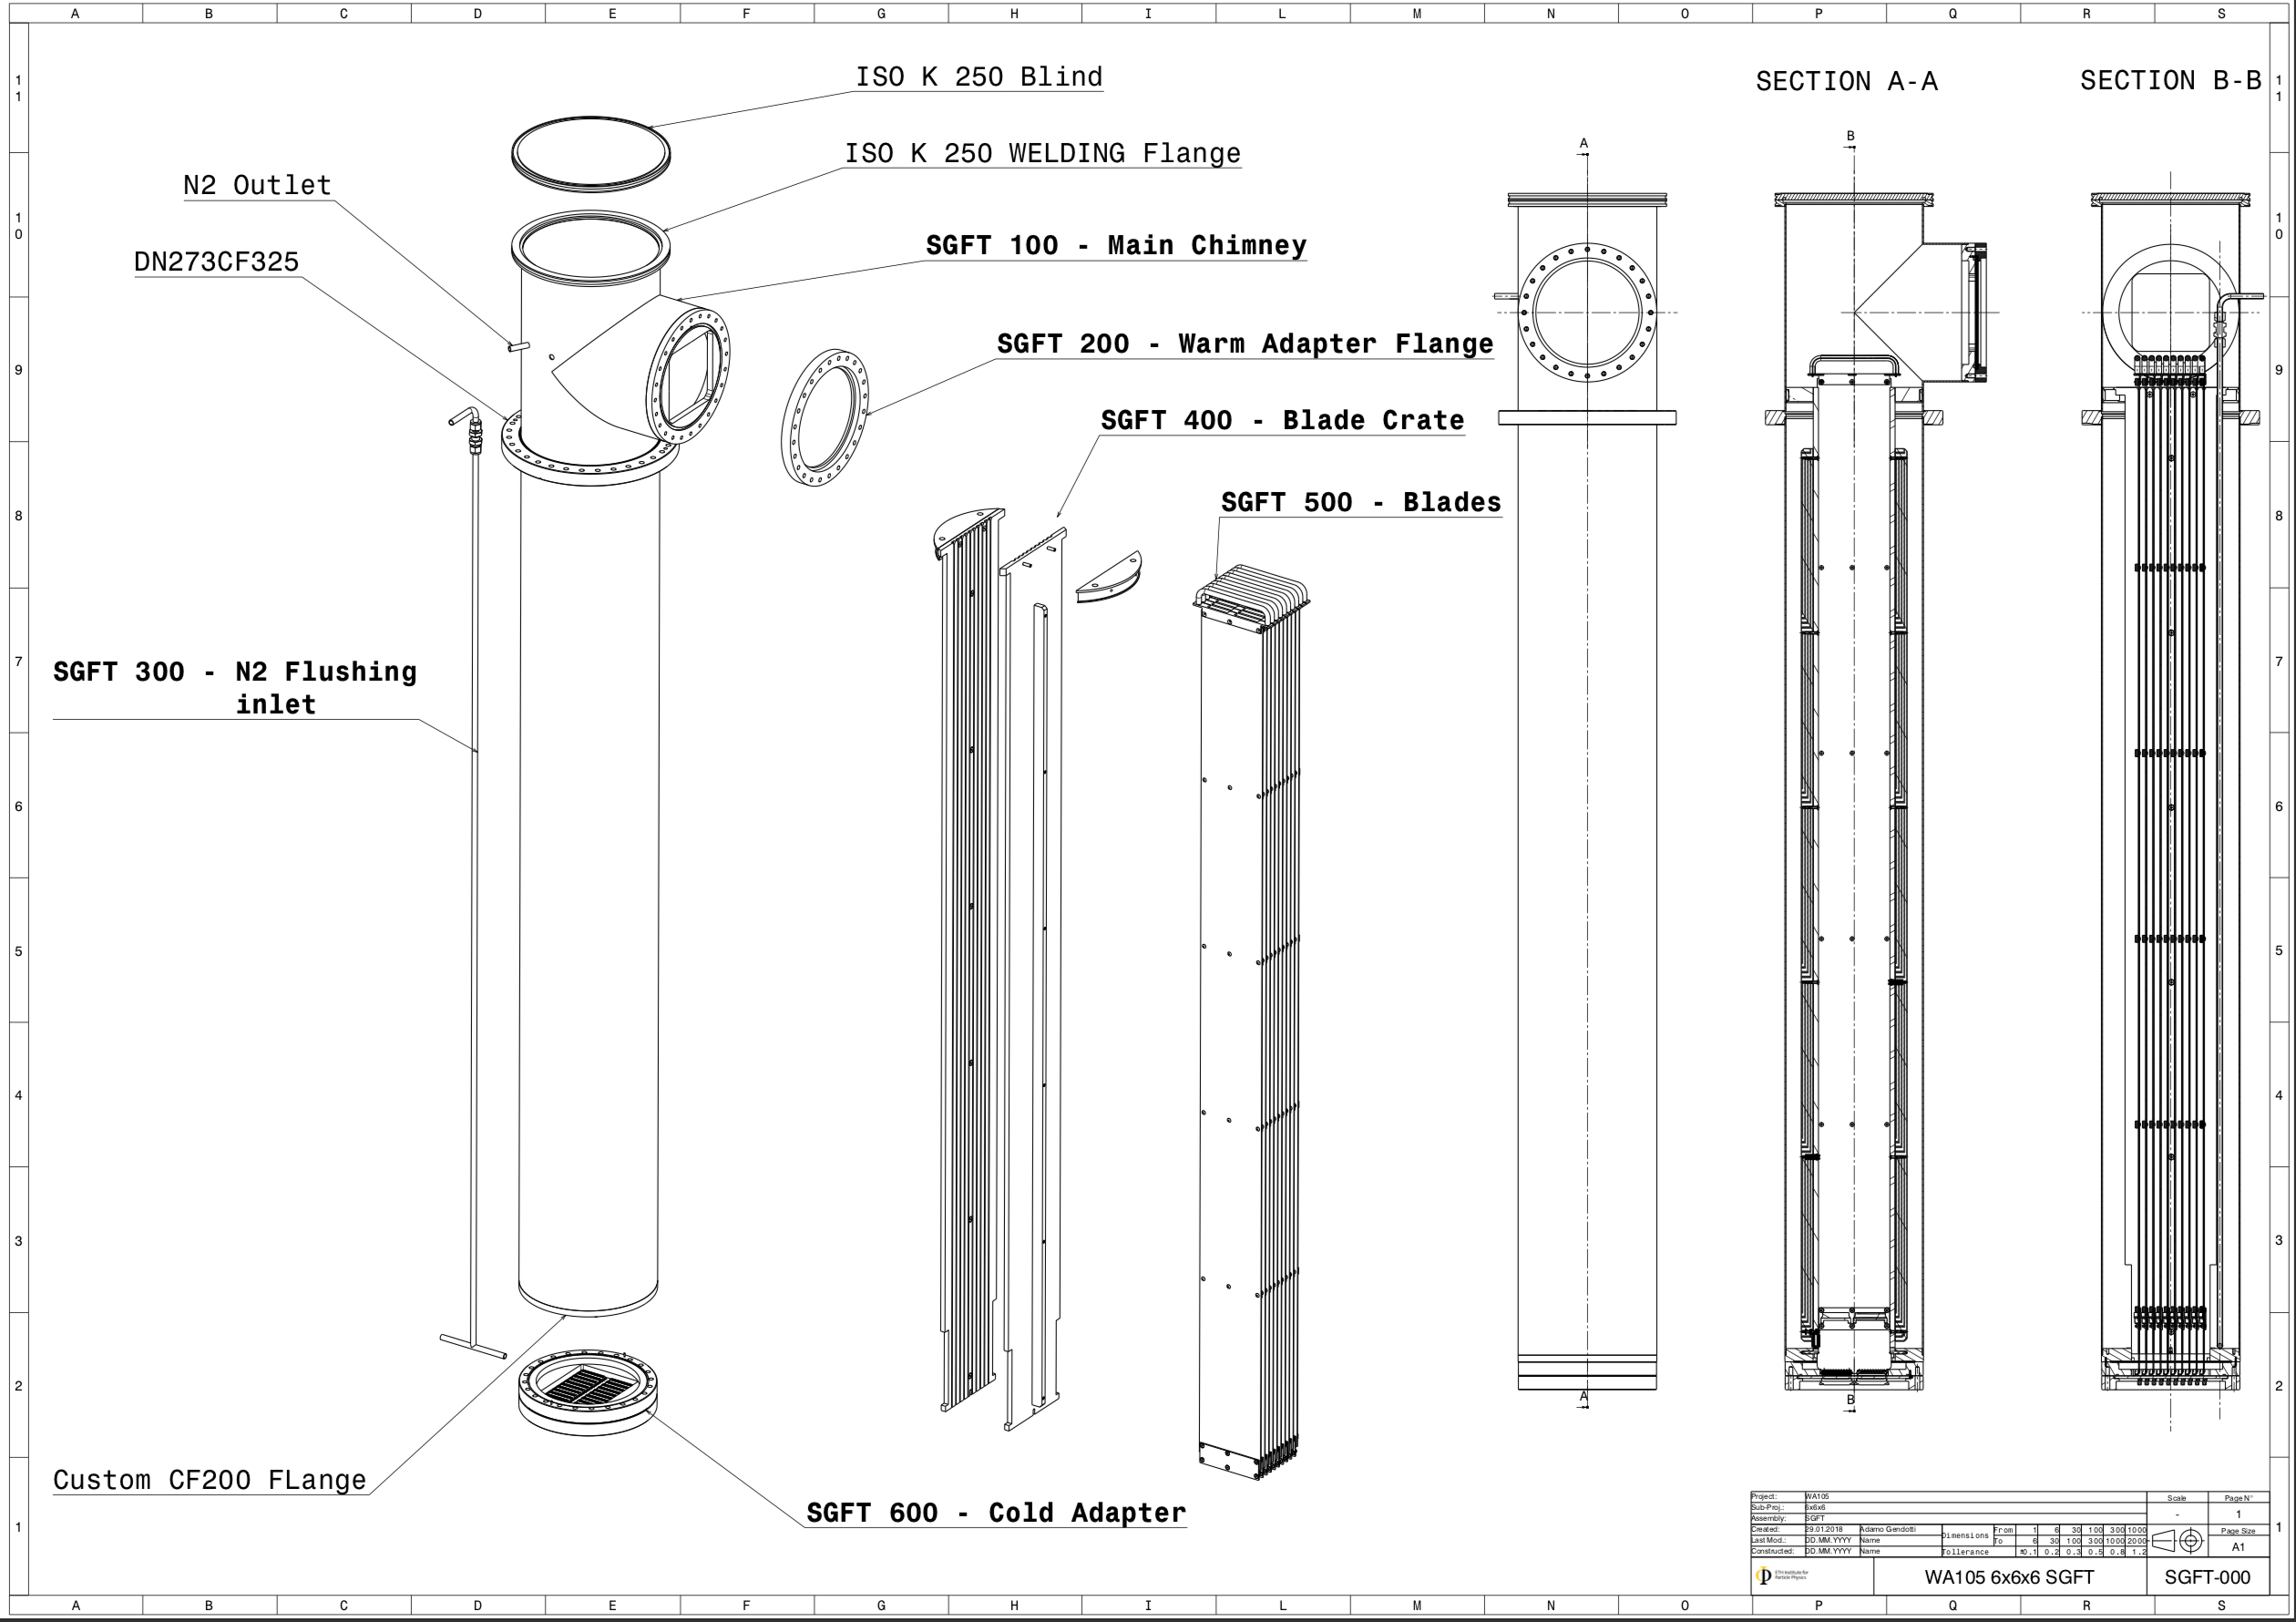
\includegraphics[width=1.\textwidth]{sgft-drawing.png}
\end{dunefigure}

The \dword{sgft} are tubes through the cryostat roof insulation.
Their inner volume is isolated form the argon and from the atmosphere.
The electronics is installed inside the tube at a level few cm below the corrugated membrane of the cryostat roof.
At the cold side of the \dword{sgft}, a flange hosts electrical connectors that connect the cables to the anode at one side and the cold electronics at the other (see figure~\ref{fig:sgft-picture}).
A system of guiding rails along the length of the \dword{sgft} ensures that the electronics can be correctly plugged into the cold flange.
\begin{dunefigure}[\dword{sgft} picture]{fig:sgft-picture}
{Image of the flange and the tube of the \dword{sgft} used in \dword{pddp} prior assembly.}
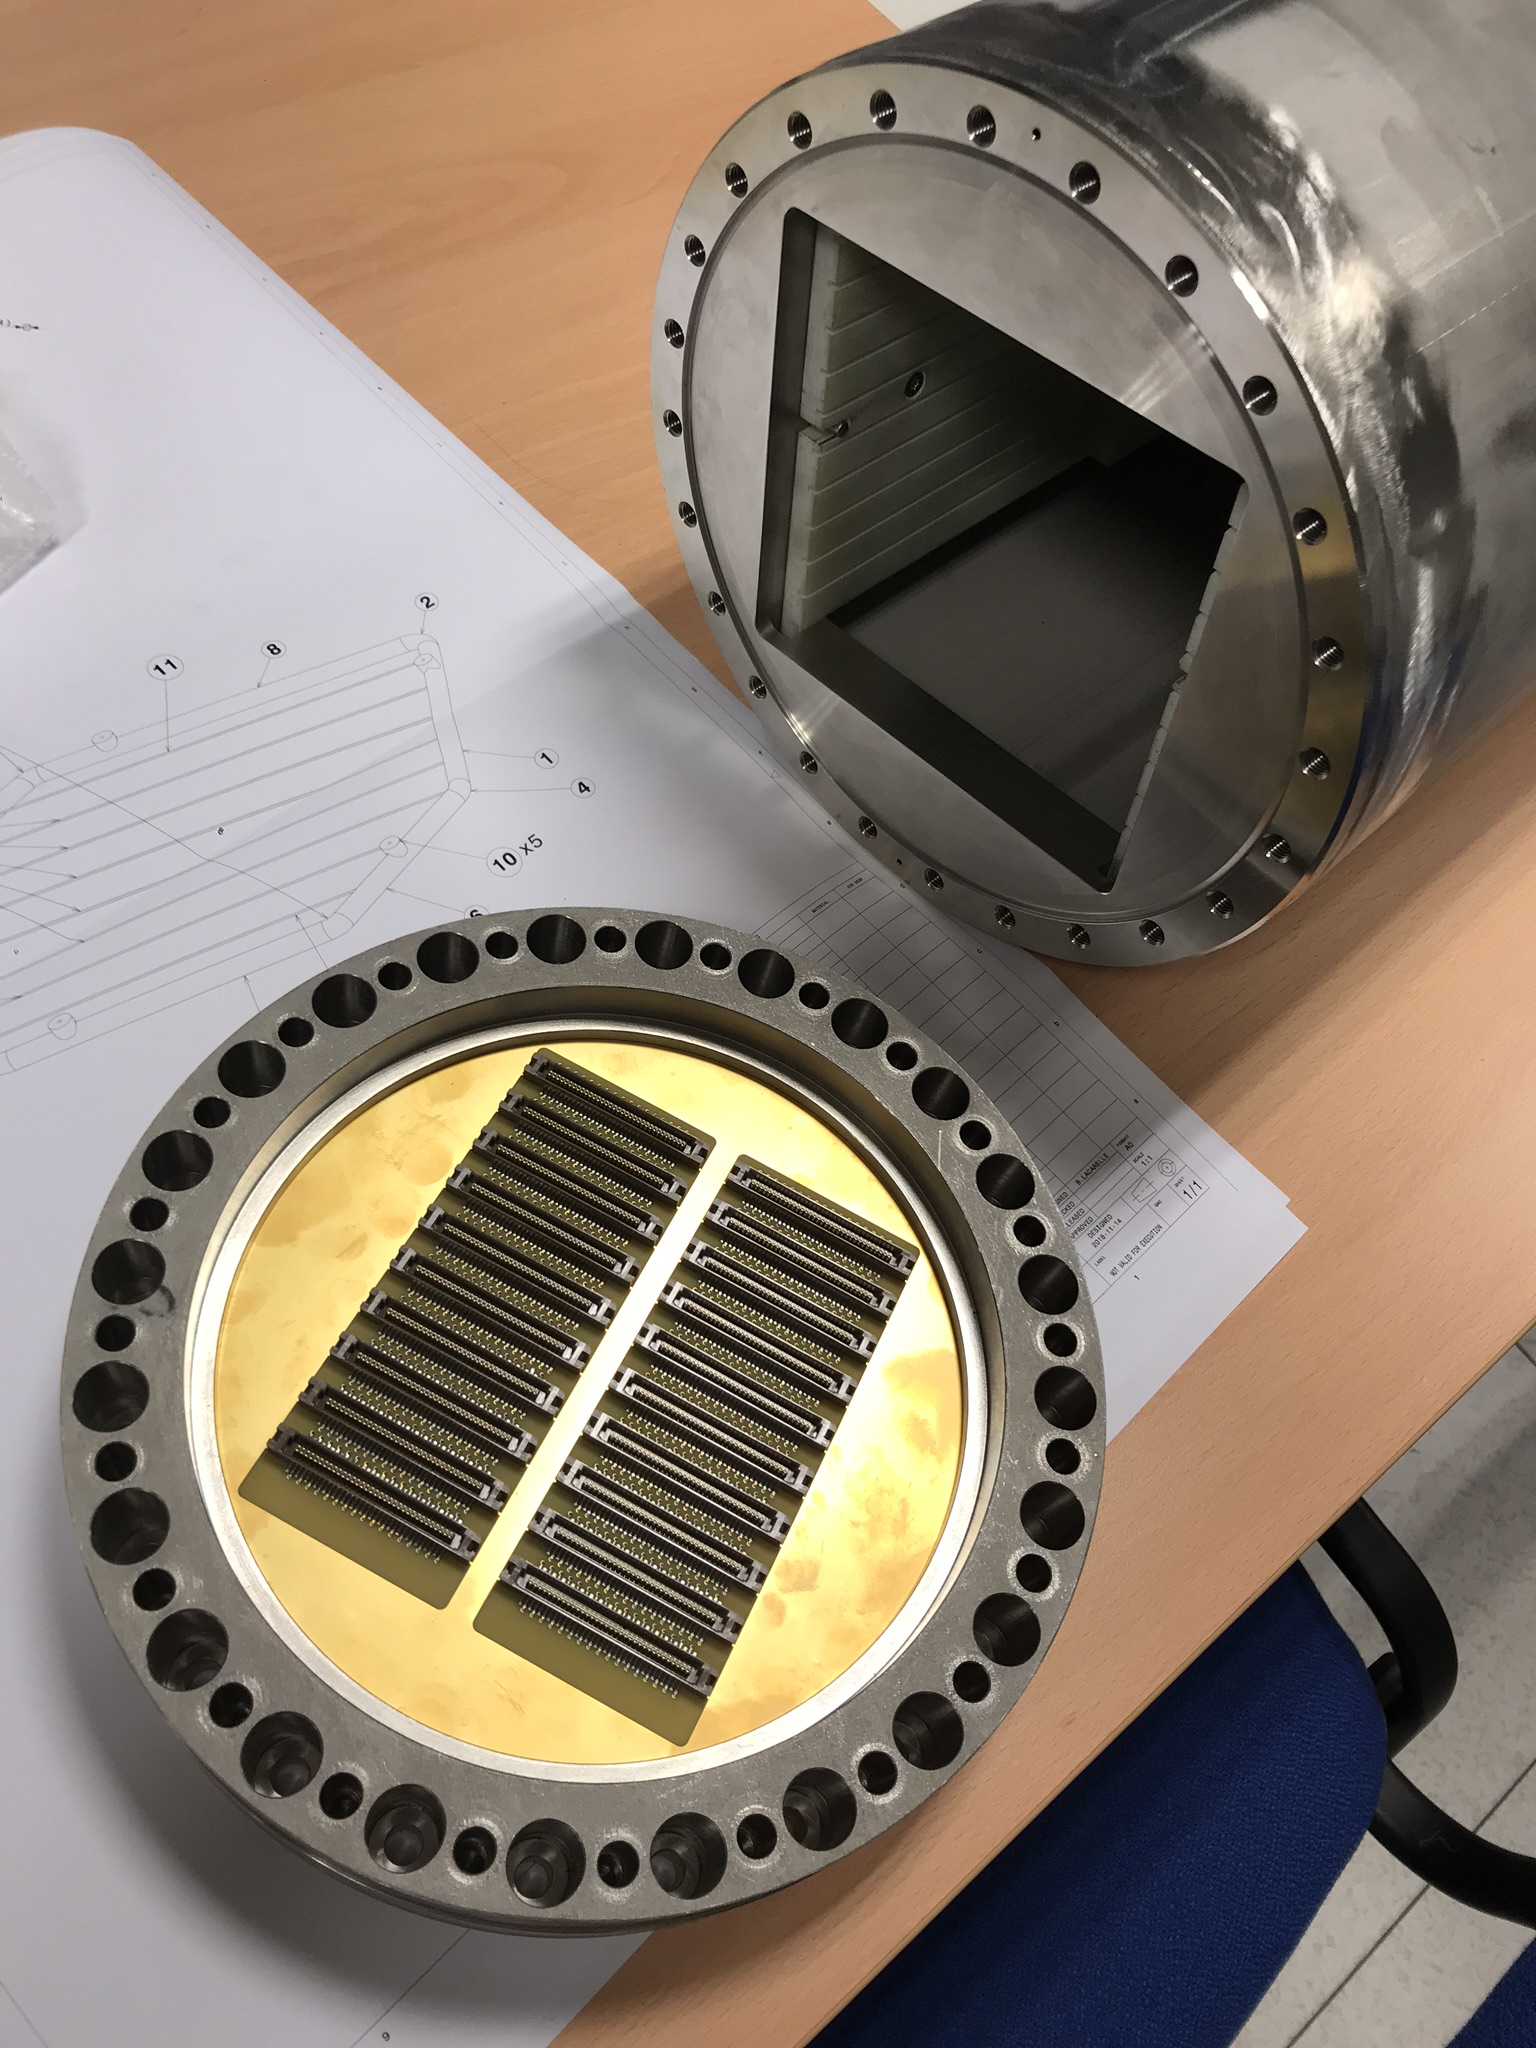
\includegraphics[width=.5\textwidth]{sgft-picture.jpg}
\end{dunefigure}
This flange is crucial because at cold it isolates the ultra-pure argon.
The \dword{sgft} volume is filled with nitrogen or argon to avoid moisture condensation on the electronics.
The temperature at the bottom of the \dword{sgft} is not low enough to allow the condensation of argon.
Having argon at 1~bar as the atmosphere inside the \dwords{sgft} would reduce the possible \dword{lar} contamination consequent to the development of a leak in the cold flange.
Each \dword{sgft} before installation must be electrically tested and helium leak must be proven to be better than $10^{-8}$~mbar$\times$l/s at room temperature.
At least the cold flanges must be leak tested at cryogenic conditions too.

DESCRIPTION OF THE LAYOUT OF THE CABLE TRAYS. NOT YET FULLY DEFINED.

DESCRIPTION OF THE LAYOUT OF THE ELECTRONICS RACKS. NOT YET FULY DEFINED.

BRIEF DESCRIPTION OF THE PURGE PIPES. SCOPE OF THE CRYOGENICS. NOTE POSSIBLE INTERFERENCES.

\subsection{Cryostat inside}
The internal cryogenics comprises manifold of pipes to ensure the proper detector purge, cool-down, filling and re-circulation of \dword{lar}.
A 3D view of the inside of the \dword{dpmod} with the cryogenic pipes is shown in figure~\ref{fig:internal-cryogenics}
All pipes enter the cryostat from the cryo penetrations on the roof.
The \dword{gar} distribution system consists of a set of pipes installed on the cryostat floor (shown in red in figure~\ref{fig:internal-cryogenics}).
These pipes are used only prior to filling to remove the air in the cryostat.
They have either a longitudinal slit or calibrated holes to distribute \dword{gar} uniformly along the length of the cryostat.
The piston purge effect was successfully tested in \dword{pdsp}.
In order to efficiently extract the air, turbulence must be avoided while purging with warm \dword{gar}.
The optimal filling speed is estimated to be 1.2~m/h (vertical height in the cryostat).
\begin{dunefigure}[Internal cryogenic piping]{fig:internal-cryogenics}
{3D model view of the internal cryogenic piping.}
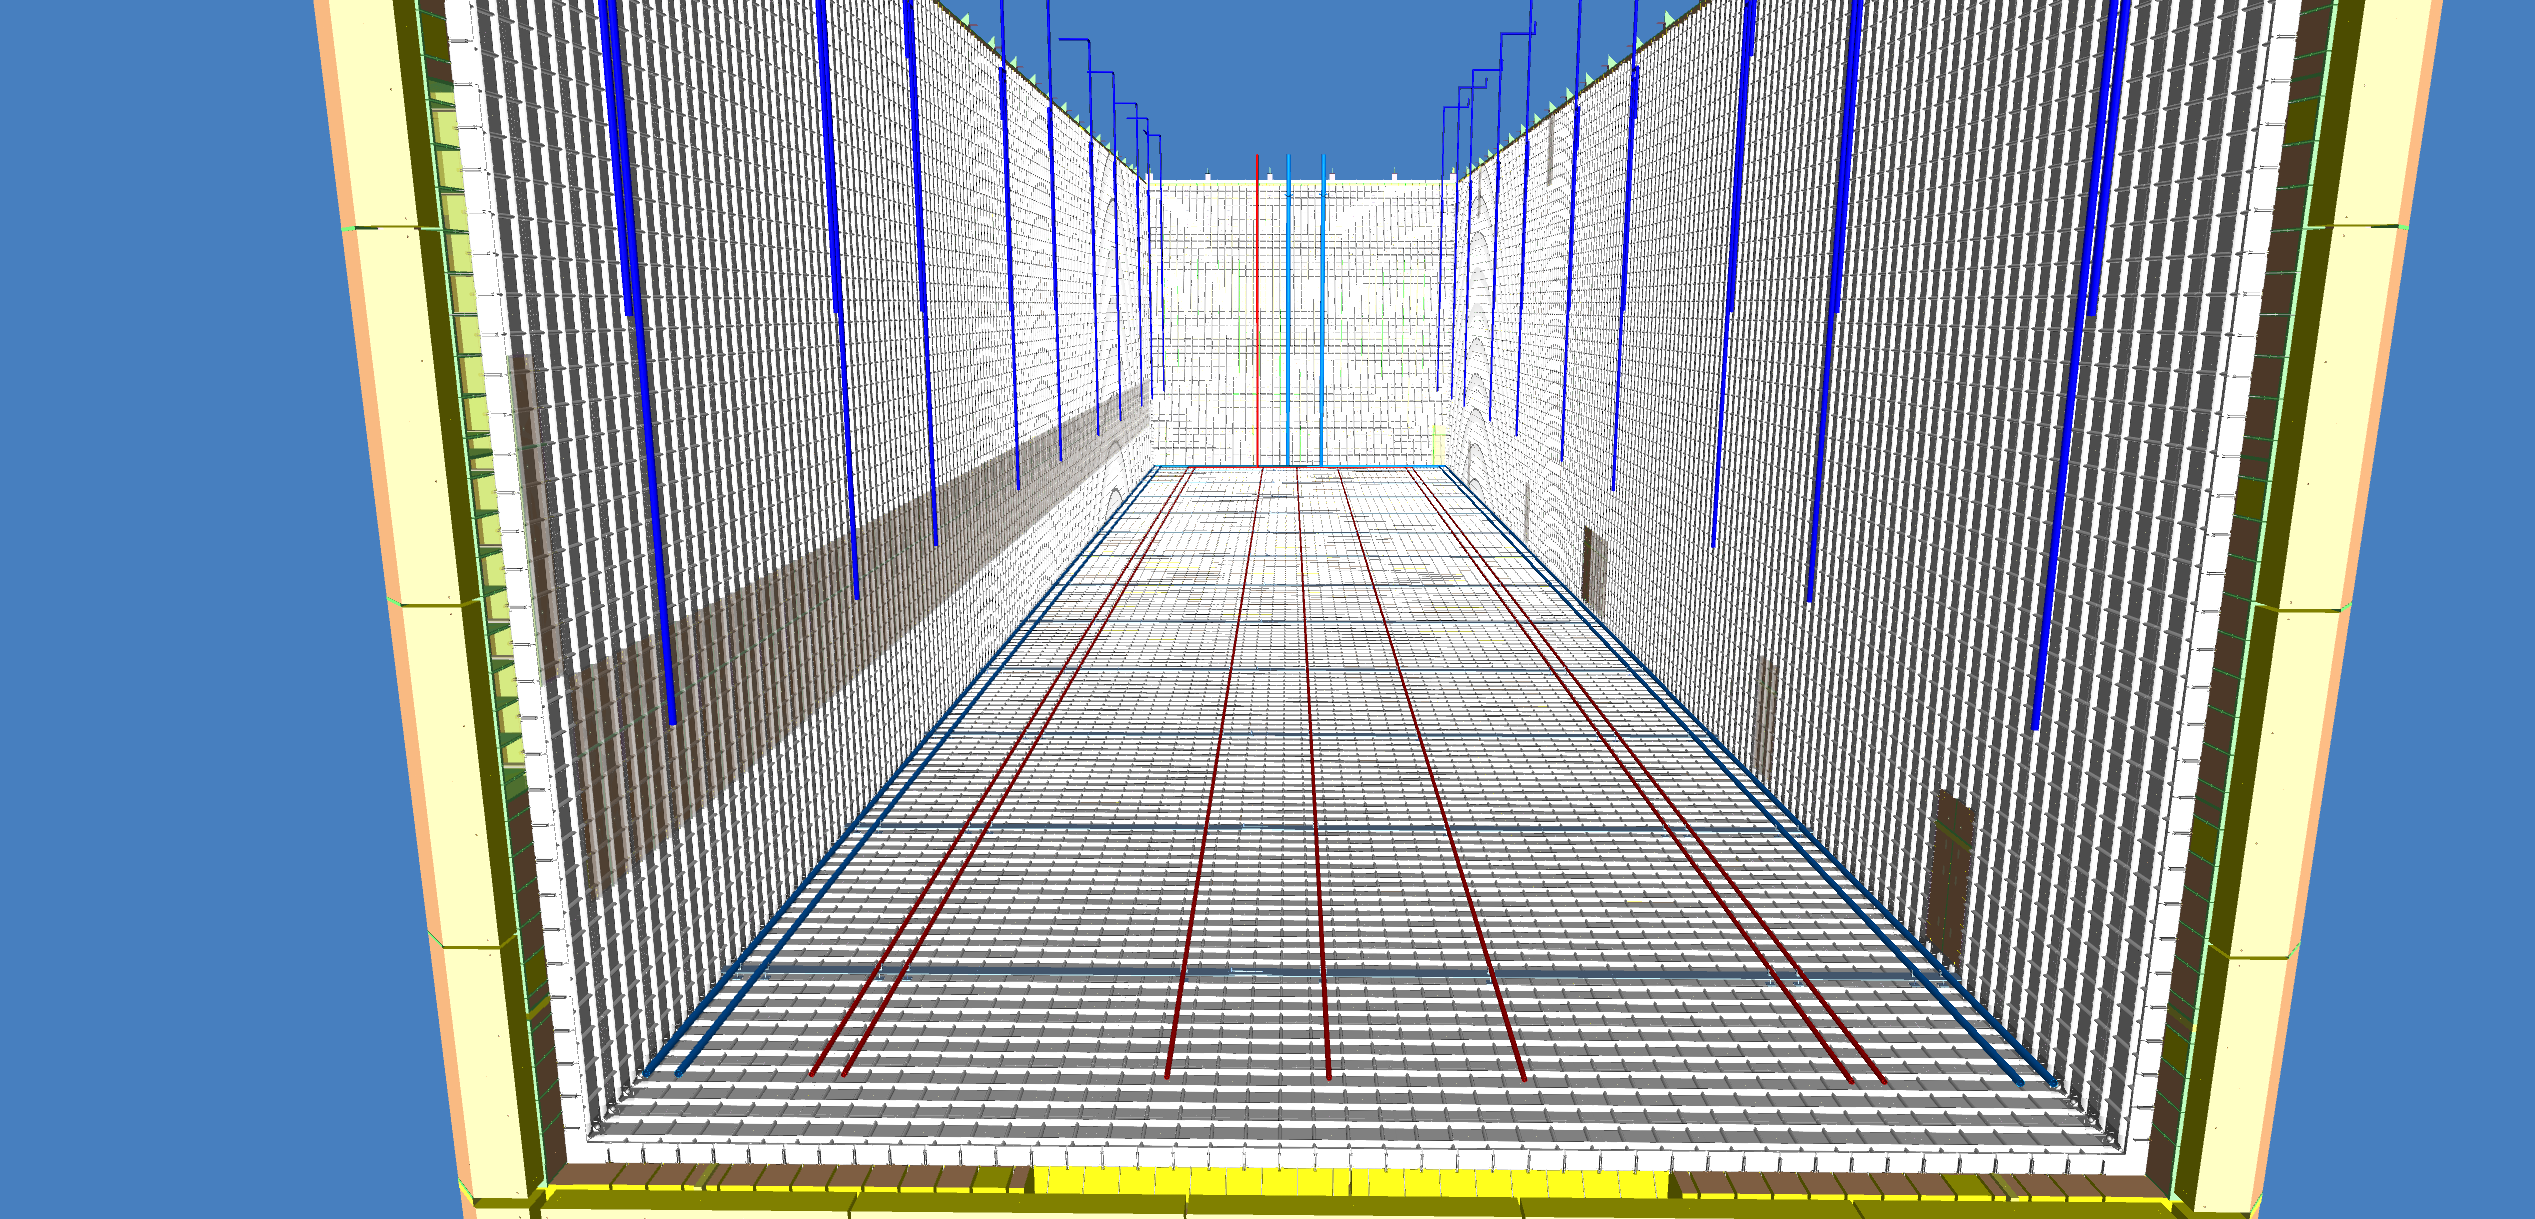
\includegraphics[width=1.\textwidth]{internal-cryogenics.png}
\end{dunefigure}

The \dword{lar} distribution system consists of a set of pipes again installed on the floor of the cryostat (shown in blue in figure~\ref{fig:internal-cryogenics}).
They are required for flowing \dword{lar} over a broad range of flow rates.
These pipes are used to fill the cryostat and, during steady state operations, to return the \dword{lar} from the purification system.
These pipes have calibrated holes to return the LAr uniformly throughout the length of the cryostat.
This is fundamental to maintain uniform purity along the full length of the detector.
Four pumps circulate the \dword{lar} inside the cryostat, all of which operate initially to achieve the desired purity.
Once the target purity is achieved, only one or two pumps remain in service.

A system of cool-down sprayers is installed along the two long walls of the cryostat just below the ceiling.
One set distributes \dword{lar} using liquid sprayers that generate a conical profile of small droplets of liquid.
The other set of sprayers distributes \dword{gar} to move the \dword{lar} droplets inside and cool down the detector and cryostat uniformly.
These sprayers are being tested \dword{pddp} and are a modified version of the ones used in \dword{pdsp}.
They are a variation of those implemented in ProtoDUNE-SP.
The cooling system design is being updated now, therefore the solution that will actually be implemented may differ from what described here.

Other infrastructure inside the cryostat includes the cryostat false floor, the UV-filtered lighting, and the battery-operated scissor lifts.
The false floor must ensure a flat surface above the internal cryogenic pipes to allow the safe operation of the man lift and the positioning of the scaffolding.
The heaviest load that the false floor must support is the 12~m high man lift, though the requirements for the false floor are not yet fully defined.
Following the experience of \dwords{protodune} the false floor can be made out of plywood panels fixed on wood blocks that defined the false floor height.
The wood blocks are simply standing on the corrugated membrane, with some plastic protection to avoid damage to the corrugated membrane.
The wood must be painted to minimise wood dust in the cryostat and it must also be treated with fire retardant agents.
The floor must be composed of section that can be independently and easily dismounted according to the needs of the installation.
This is fundamental when installing the \dword{pd} and the ground grid, since they occupy the space taken by the false floor.

The cryostat lighting, using UV-filtered LED lamps, is expected to be fairly simple.
Options for the lighting will be developed further during tests at the Ash River facility.
Floor-mounted lights and lights entering from some roof penetrations will be investigated.

At least one commercially-available battery-operated scissor lift with a 12~m reach is used to work on the \dword{crp} installation and cabling as well as for the installation of the field cage and the cryogenic instrumentation.
Tests at Ash River will verify the stability of the lift at height.
If the lift is determined to be suitable, then the remaining issue to resolve is how to insert and remove it from the cryostat.
Commercially-available scissor lifts are too wide to fit easily through the \dword{tco} opening where one of the large cryostat support I-beams protrudes above the floor level.
Custom lifting equipment is needed to insert and remove the lifts into the cryostat.
At the end of the installation process, the last lift may require partial dismantling before it can be removed from the cryostat.

VENTILATION

\subsection{Clean room}
The underground clean room in front of the \dword{tco} is the main place where the detector components are unpacked, assembled and tested prior the installation inside the cryostat.
The experience in building \dword{pdsp} and \dword{pddp} showed that the role of the clean room is fundamental in several aspects.
The cleanliness of the air and the absence powder and dust is fundamental for all the detector components, and in particular for the \dwords{lem} in the \dwords{crp}.
The clean room should ensure the adequate cleanliness of the air where the detector components are unpacked and tested, and it should meet ISO-8 clean room class standards.
The clean room also isolates and protects the inside of the cryostat from the dirty environment of the cavern, which has exposed exposed rocks and non-protected floor.
In order to achieve this, a ventilation and an air filtration system well dimensioned is required.
The requirements for work in an ISO-8 cleanroom are a cleanroom lab coat, clean shoes, or shoe-covers, and nets for hair and beards.
This is in addition to a clean hard hat and gloves for safety reasons.

The clean room must provide space and tools to test the detector equipment, most notably the \dwords{crp} in the cold boxes and the \dword{pmt} tests in the dark box.
Compared to the \dword{spmod} the clean room is smaller in all the directions, since most components do not need to be assembled prior installation, and the major assembly work of the cathode and field cage is done directly inside of the cryostat.

Two view of the 3D model of the clean room are shown in figure~\ref{fig:cleanroom}.
The clean room surrounds and seals against the \dword{tco}, to isolate the cryostat.
In addition, the cryostat \dword{tco} can be temporary closed with plastic curtains, to isolate it from possible dirty jobs inside the clean room.

THE DP TCO IS SMALLER BUT THE MODEL IS NOT YET UPDATED

The mechanical structure for the clean room is a self sustained steel skeleton where the walls, made out of rigid aluminium-foam-aluminium sandwich panels, are fixed.
The size of the clean room are about $16 \mathrm{(L)} \times 16 \mathrm{(L)} \times 9 \mathrm{(H)}$~m$^3$.
The floor must be covered with resin or other material that is simple to keep clean.
The clean room floor and the objects inside the clean room must undergo regular cleaning in order to ensure all the time the ISO-8 class standard.

\begin{dunefigure}[Internal cryogenic piping]{fig:cleanroom}
{Two views of the 3D model of the clean room in front of the \dword{tco}.}
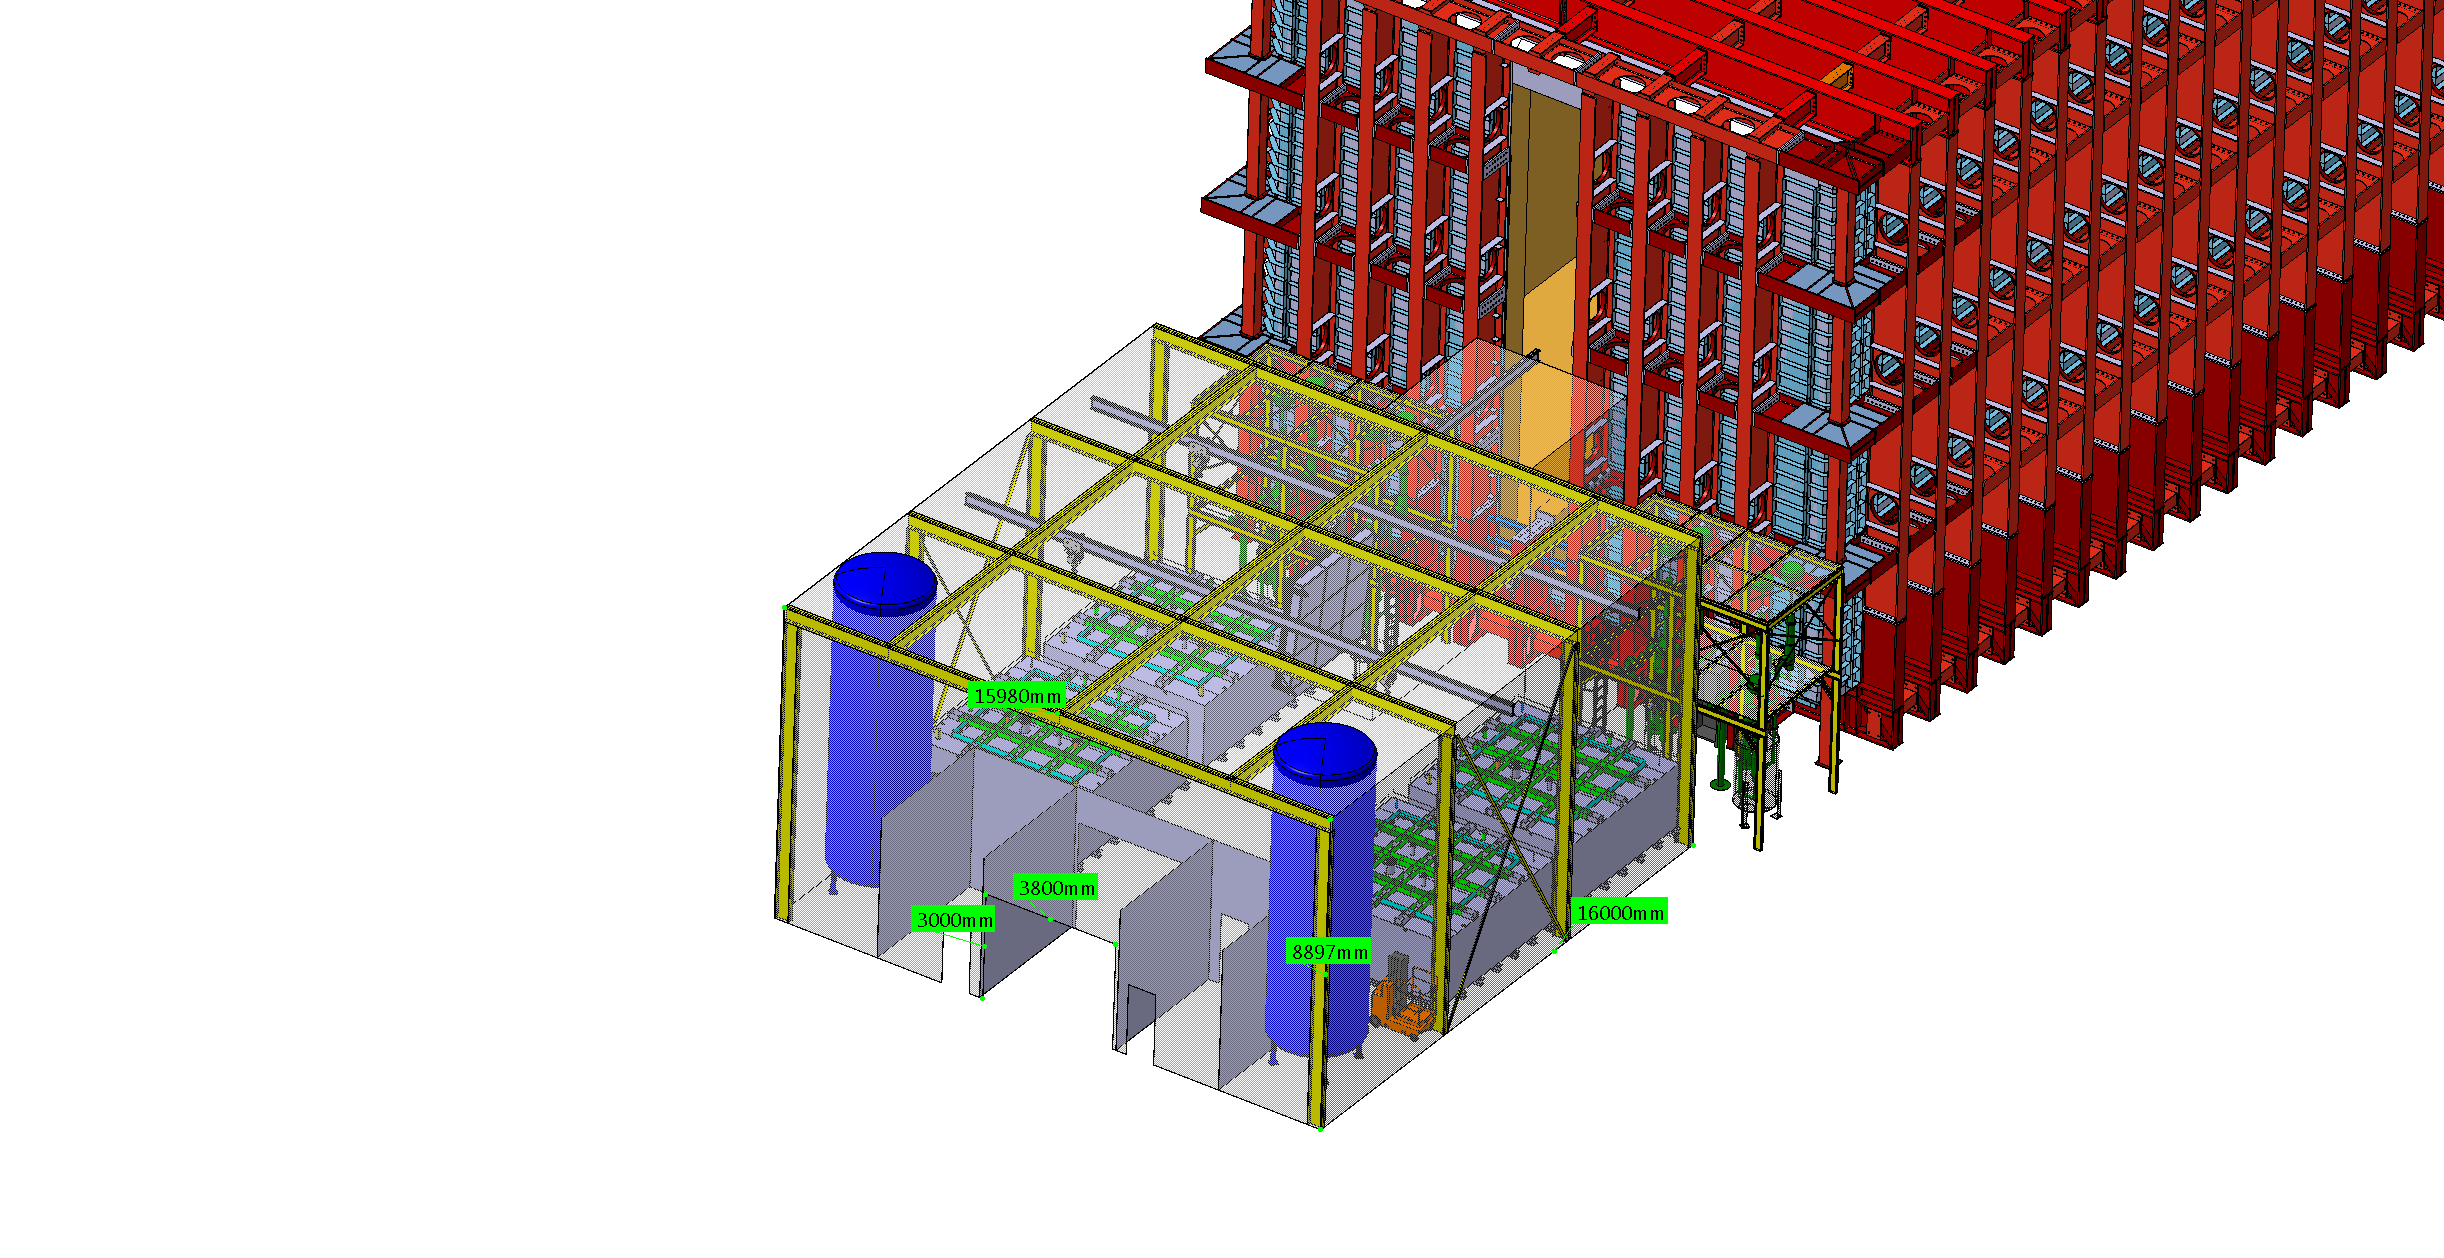
\includegraphics[width=1.\textwidth]{cleanroom1.png}
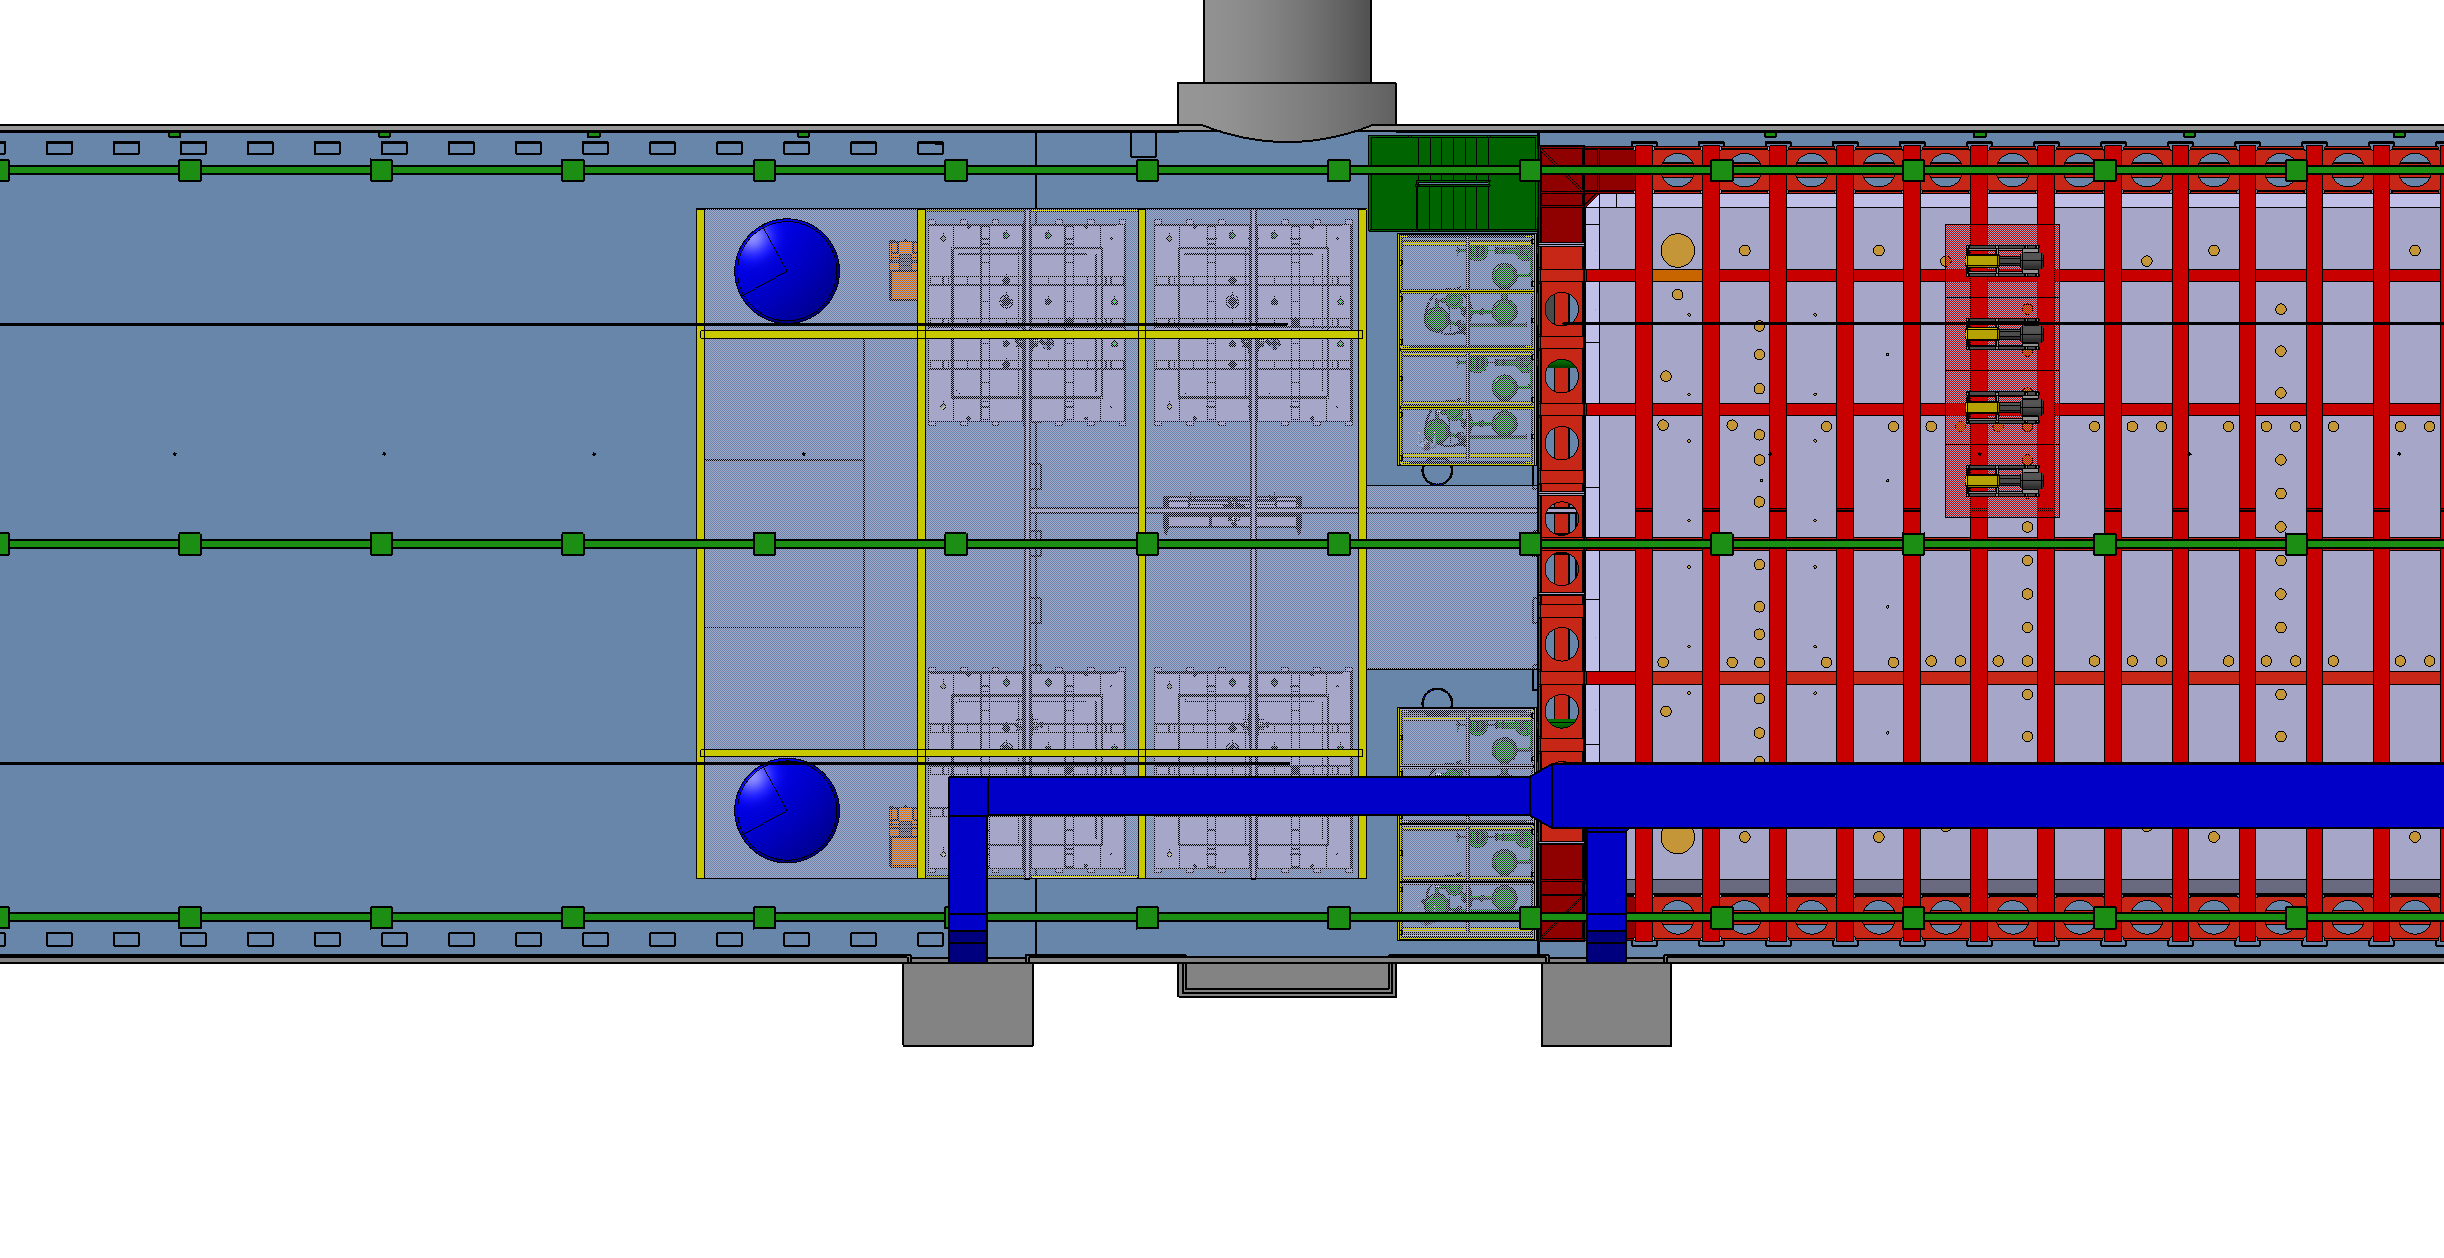
\includegraphics[width=1.\textwidth]{cleanroom2.png}
\end{dunefigure}

The clean room layout can be seen in figure~\ref{fig:cleanroom} (bottom).
Around the \dword{tco} enough space is left in order to install and access the four liquid argon pumps that stay on the cryostat level on the two sides of the \dword{tco}.
The clean room is equipped with four cold boxes, overhead mobile cranes, a material airlock, a personnel airlock, space for the cryogenics to operate the cold boxes, and a room to test the \dwords{pmt} in a dark box.
Additional space may be required to work on detector components that need to be modified/fixed/refurbished and for which the work does not justify to bring the component on surface.
An additional $5\times6$~m$^2$ equipped with two gantry cranes to lift one \dword{crp} may be needed and can be foreseen.
The material airlock is large enough to house one \dword{crp} box, that is the widest component that needs to enter.
The material access is done at the cryostat level through two 3.8~m large rolling doors.
Unlike the \dword{pdsp} and \dword{pddp}, in this cans the airlock does not need to have an openable roof.
Nonetheless, this option can be easily implemented in the present design of the clean room.
In this airlock the material is cleaned and if needed unpacked before entering into the actual clean room.
For the components that are longer than the length of the airlock, as possibly the I beam that support the filed cage, both the doors can be temporary and shortly opened to allow the access of the material without compromise the quality of the air in the clean room.
In case of longer operation that require both rolling doors to be opened, temporary plastic curtains can be installed to limit the powder and dust from the cavern to enter into the clean room.
The airlock is large enough so that a standard fork-lift can enter and maneuver.
Inside the cleanroom, instead, due to space constraints only manual forklift can be used.

The clean room hosts four cold boxes and the cryogenic infrastructure in order to operate them.
The cold boxes are arranged in two rows along the walls of the clean room, one in front of the other.
The central region is used to manipulate the \dword{crp} box and to attach the \dword{crp} below the cold box roof.
This region is also used to manipulate all the elements prior insertion in the cryostat.

The cryogenics for the cold boxes is not fully defined and detailed yet.
The tall cryostats shown in figure~\ref{fig:cleanroom} are mostly a place-holder.
If more space is required for the cryogenic installation, the area outside the clean room can be used, since the cryogenics does not need to be installed in a clean environment.

Along the width of the clean room and above the cold boxes there are I-beams equipped with trolleys and electrical hoists that serve as 2~ton over-head cranes to open and close the cold boxes.
These I beams may be connected to the cavern walls or the steel structure of the clean room.
A third I-beam connects the \dword{tco} structure to the clran room structure and in the same way it is used as crane to bring material inside the cryostat.
The heaviest detector component to be brought inside the cryostat is the \dword{crp} in its box.
Its total weight is below 800~kg.
No major activities at height are needed inside the clean room.
For the lifting of the \dword{crp} box and in order to insert it inside the cryostat there will be available at least one 8~m-tall compact man lift.

The \dword{crp} in its box is not the heavies object to enter into the cryostat.
In fact, despite not having yet identified the 12~m tall man lift, it will certainly be heavier and bigger than the \dword{crp} box.
A custom tool to insert heavy object inside the cryostat must be developed and possibly to be used in conjunction to the cavern crane.
For this reason, the clean room roof in front of the \dword{tco} and the I-beam that enters into the cryostat can be removed.
This operation will be necessary also to complete the closure of the external structure of the \dword{tco}.

CABLE TRAYS

\subsection{Cold boxes}
An electrical and mechanical test of each entire \dword{crp} in realistic cryogenic thermodynamic conditions and in reasonably pure argon vapor must be performed in order to access the final \dword{qc} of the \dword{lem} and \dword{crp} assembly before the installation in the cryostat.

The tests are performed in four dedicated cryostats, also referred to as \emph{cold boxes}, installed in the clean room in front of the \dword{tco} and with dedicated cryogenic infrastructure that allows to operate each of them independently.
The objectives of the global test of the \dwords{crp} are:
\begin{itemize}
\item the characterization of the \dword{hv} operation of each \dword{lem} independently and as well the \dword{hv} operation of all the 36~\dwords{lem} forming a \dword{crp} at the same time,
\item the characterization of the \dword{hv} operation of the extraction grid,
\item the test of all the \dword{hv} contacts from the feedthroughs to the \dword{lem} and grid connectors,
\item the measurement of the flatness of the \dword{crp} during the test and the capability to align the \dword{crp} to the \dword{lar} level.
\item calibration of the level measurement from the capacitance between the extraction grid and the bottom electrode of the \dword{lem}.
\end{itemize}

The requirements for the environment of this test are defined as following:
\begin{itemize}
\item the \dword{lar} surface must be flat withing 2~mm in order to allow the \dword{lem} to be in the vapor phase and the grid in liquid phase,
\item the vapor pressure does not need to be stabilised, but it must constantly be monitored,
\item the vapor temperature should not be controlled, but constantly monitored,
\item the liquid argon purity should be of the order of at most 100~ppm (O$_2^{eq}$), in order to be comparable with the tests at 3.3~bar and room temperature done for each \dword{lem} during the \dwords{qc} before reaching \surf,
\item the \dword{crp} vertical position and horizontality should be adjustable, at least before the filling of the cold box.
\end{itemize}

Figure~\ref{fig:NP02-ColdBoxSketch} shows a sketch of the cold box.
The same concept of cold box was successfully used several times at \dword{cern} in 2018 to characterise the four \dwords{crp} installed in \dword{pddp}.
\begin{dunefigure}[Sketch of the cold box]{fig:NP02-ColdBoxSketch}
{Schematic representation of one cold box for the test of the \dwords{crp}.}
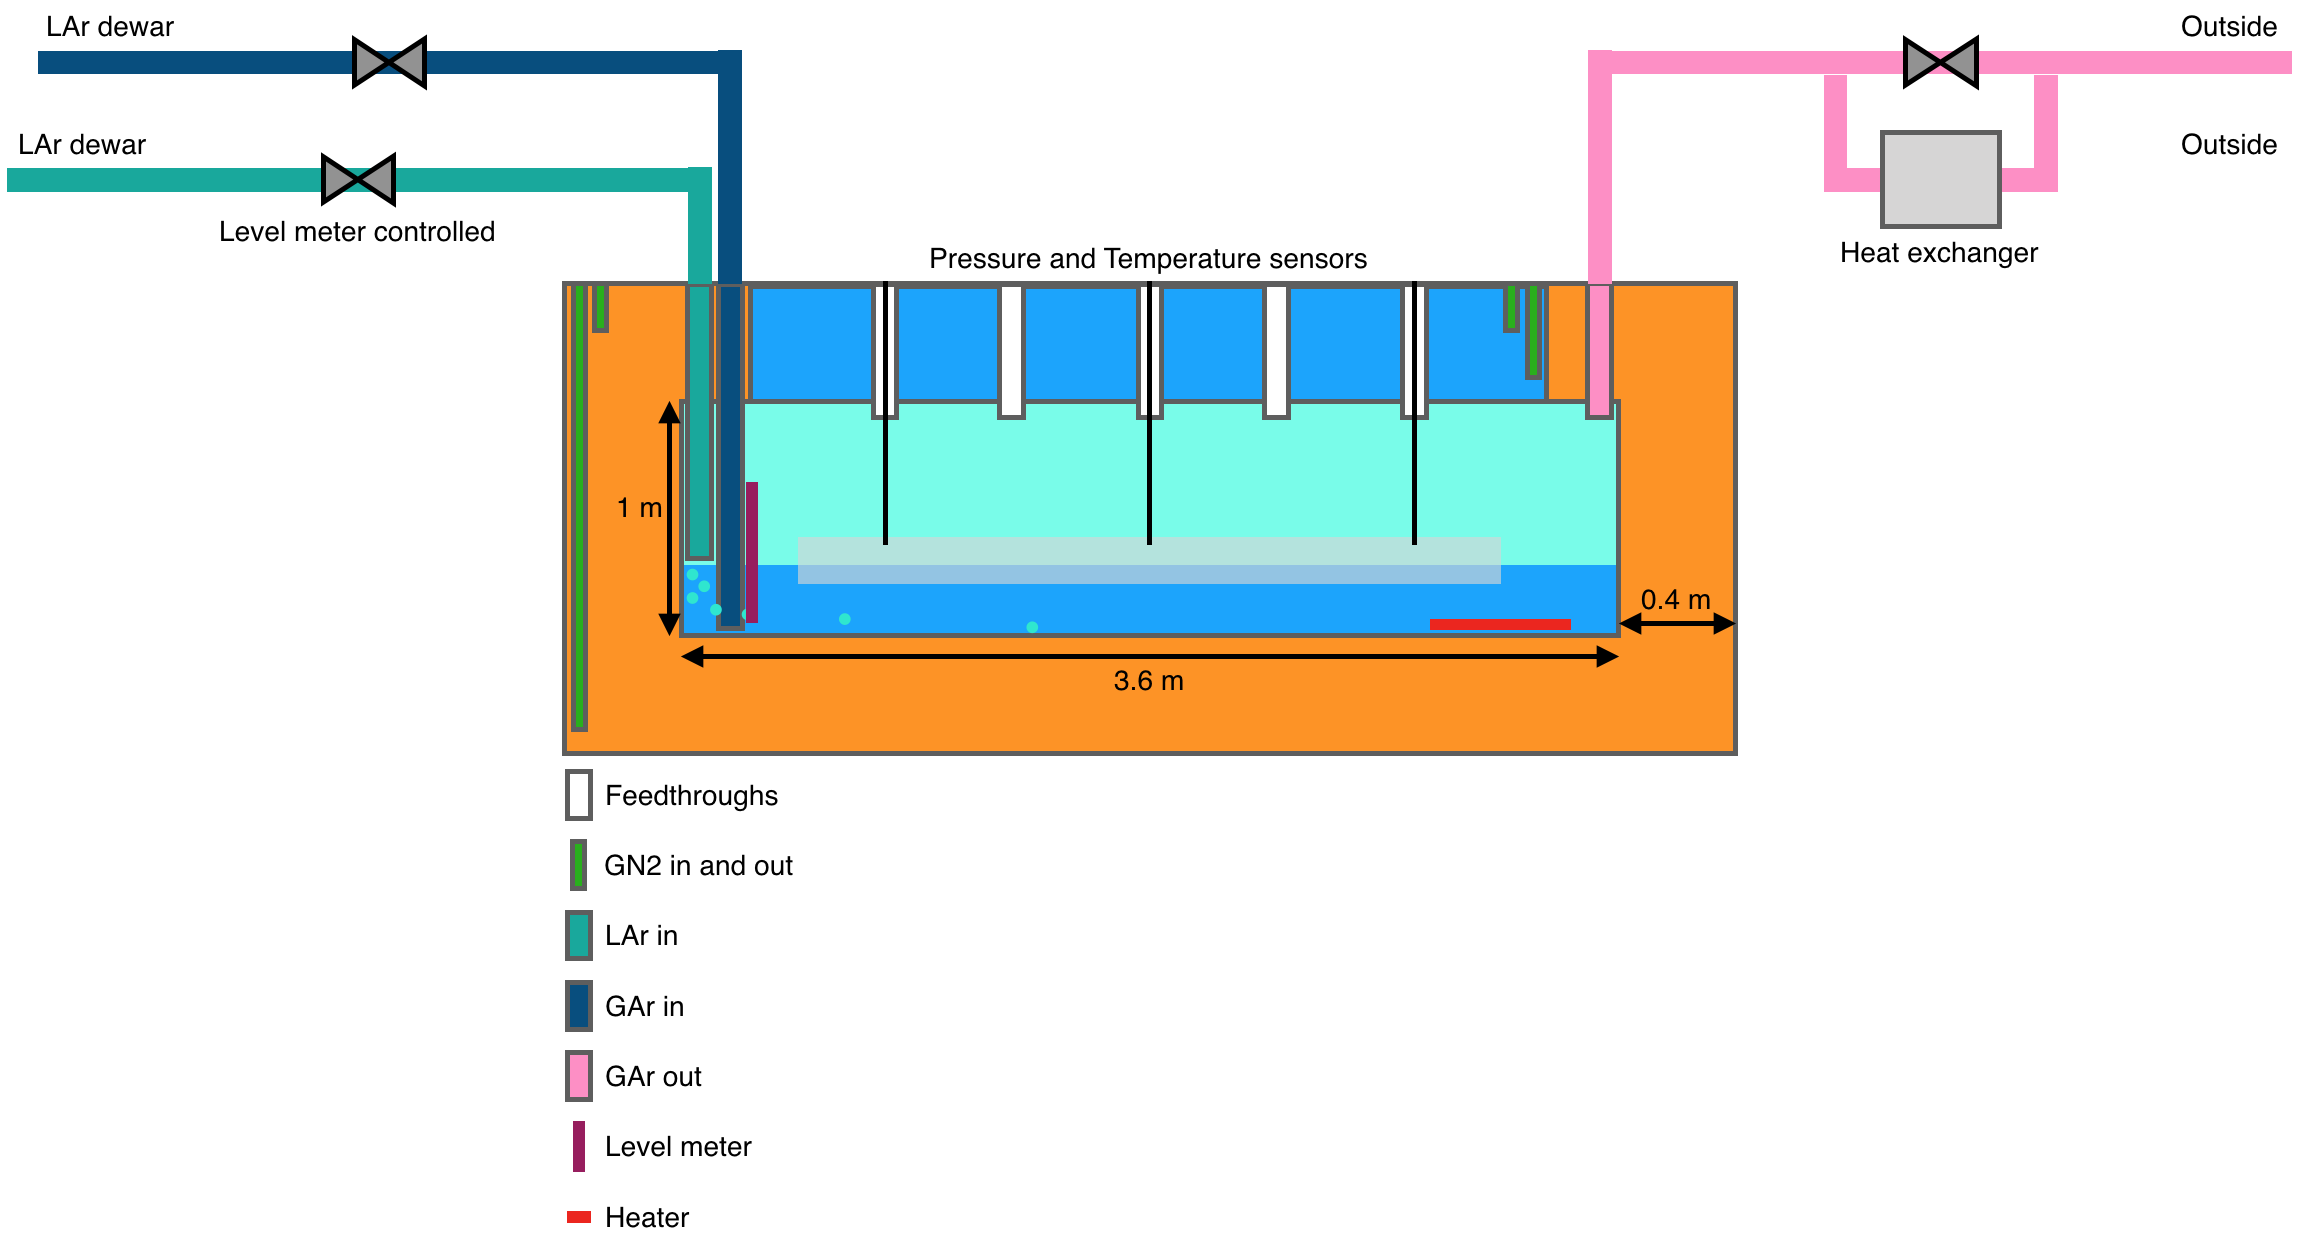
\includegraphics[width=1.\textwidth]{NP02-ColdBoxSketch.png}
\end{dunefigure}
The external structure is a self-sustained box made out of 1~cm-thick stainless steel plates.
The internal membrane is made out of 2~mm-thick stainless steel plates.
The internal dimensions are 1~m in height and 3.9~m in the other directions.
The thermal insulation is passive and it consists of four layers each of 10~cm-thick polyurethane foam (30~kg/m$^3$).
The insulation layers are separated by polyethylene foils to minimise the convection phenomena and the consequent increase of heat input.
The insulation region is flushed with gas nitrogen, as it is done for all the corrugated membrane cryostats.
The cold boxes are too large to be transported underground, therefore they must be produced underground during the construction of the clean room.
A custom made RGA-based dense gas analyser monitors the composition of the gas nitrogen circulating in the insulation space.
The same system may be used to monitor the quality of argon boil-off with a sensitivity of about 50~ppm of O$_2$ and N$_2$.

The \dwords{crp} is attached to a portion of the roof (shown in blue in figure~\ref{fig:NP02-ColdBoxSketch}) that can be opened.
The horizontality and the vertical position of the \dword{crp} can be adjusted withing $\pm 20$~mm around the nominal position.
The adjustment is done manually from the hanging system installed on the roof.
In order to empty the box once the test is concluded, a 10~kW heater is used to evaporate the liquid argon, that is then re-condensed by the cryogenic system and stored in a standard insulated cryostat.

The liquid argon level in the cold box is kept constant by compensating the losses due to the evaporation with new liquid argon.
The cold boil-off vapour is sent to the cryogenic systems via vacuum insulation pipes to be re-condensed.

DESCRIPTION OF THE CRYO SYSTEM REQUIREMENTS

CYCLE DESCRIPTION

The operation of the \dword{pddp} cold box proved that the requirements can be met and exceeded.
Figure\ref{fig:NP02-cold-box} shows the \dword{pddp} cold box prior being closed for a test.
A \dwords{crp} is hanging from the roof and it is being closed inside the box.
\begin{dunefigure}[Photo of the \dword{pddp} cold box]{fig:NP02-cold-box}
{Photo of the \dword{pddp} cold box open and with a \dwords{crp} hanging from the roof.}
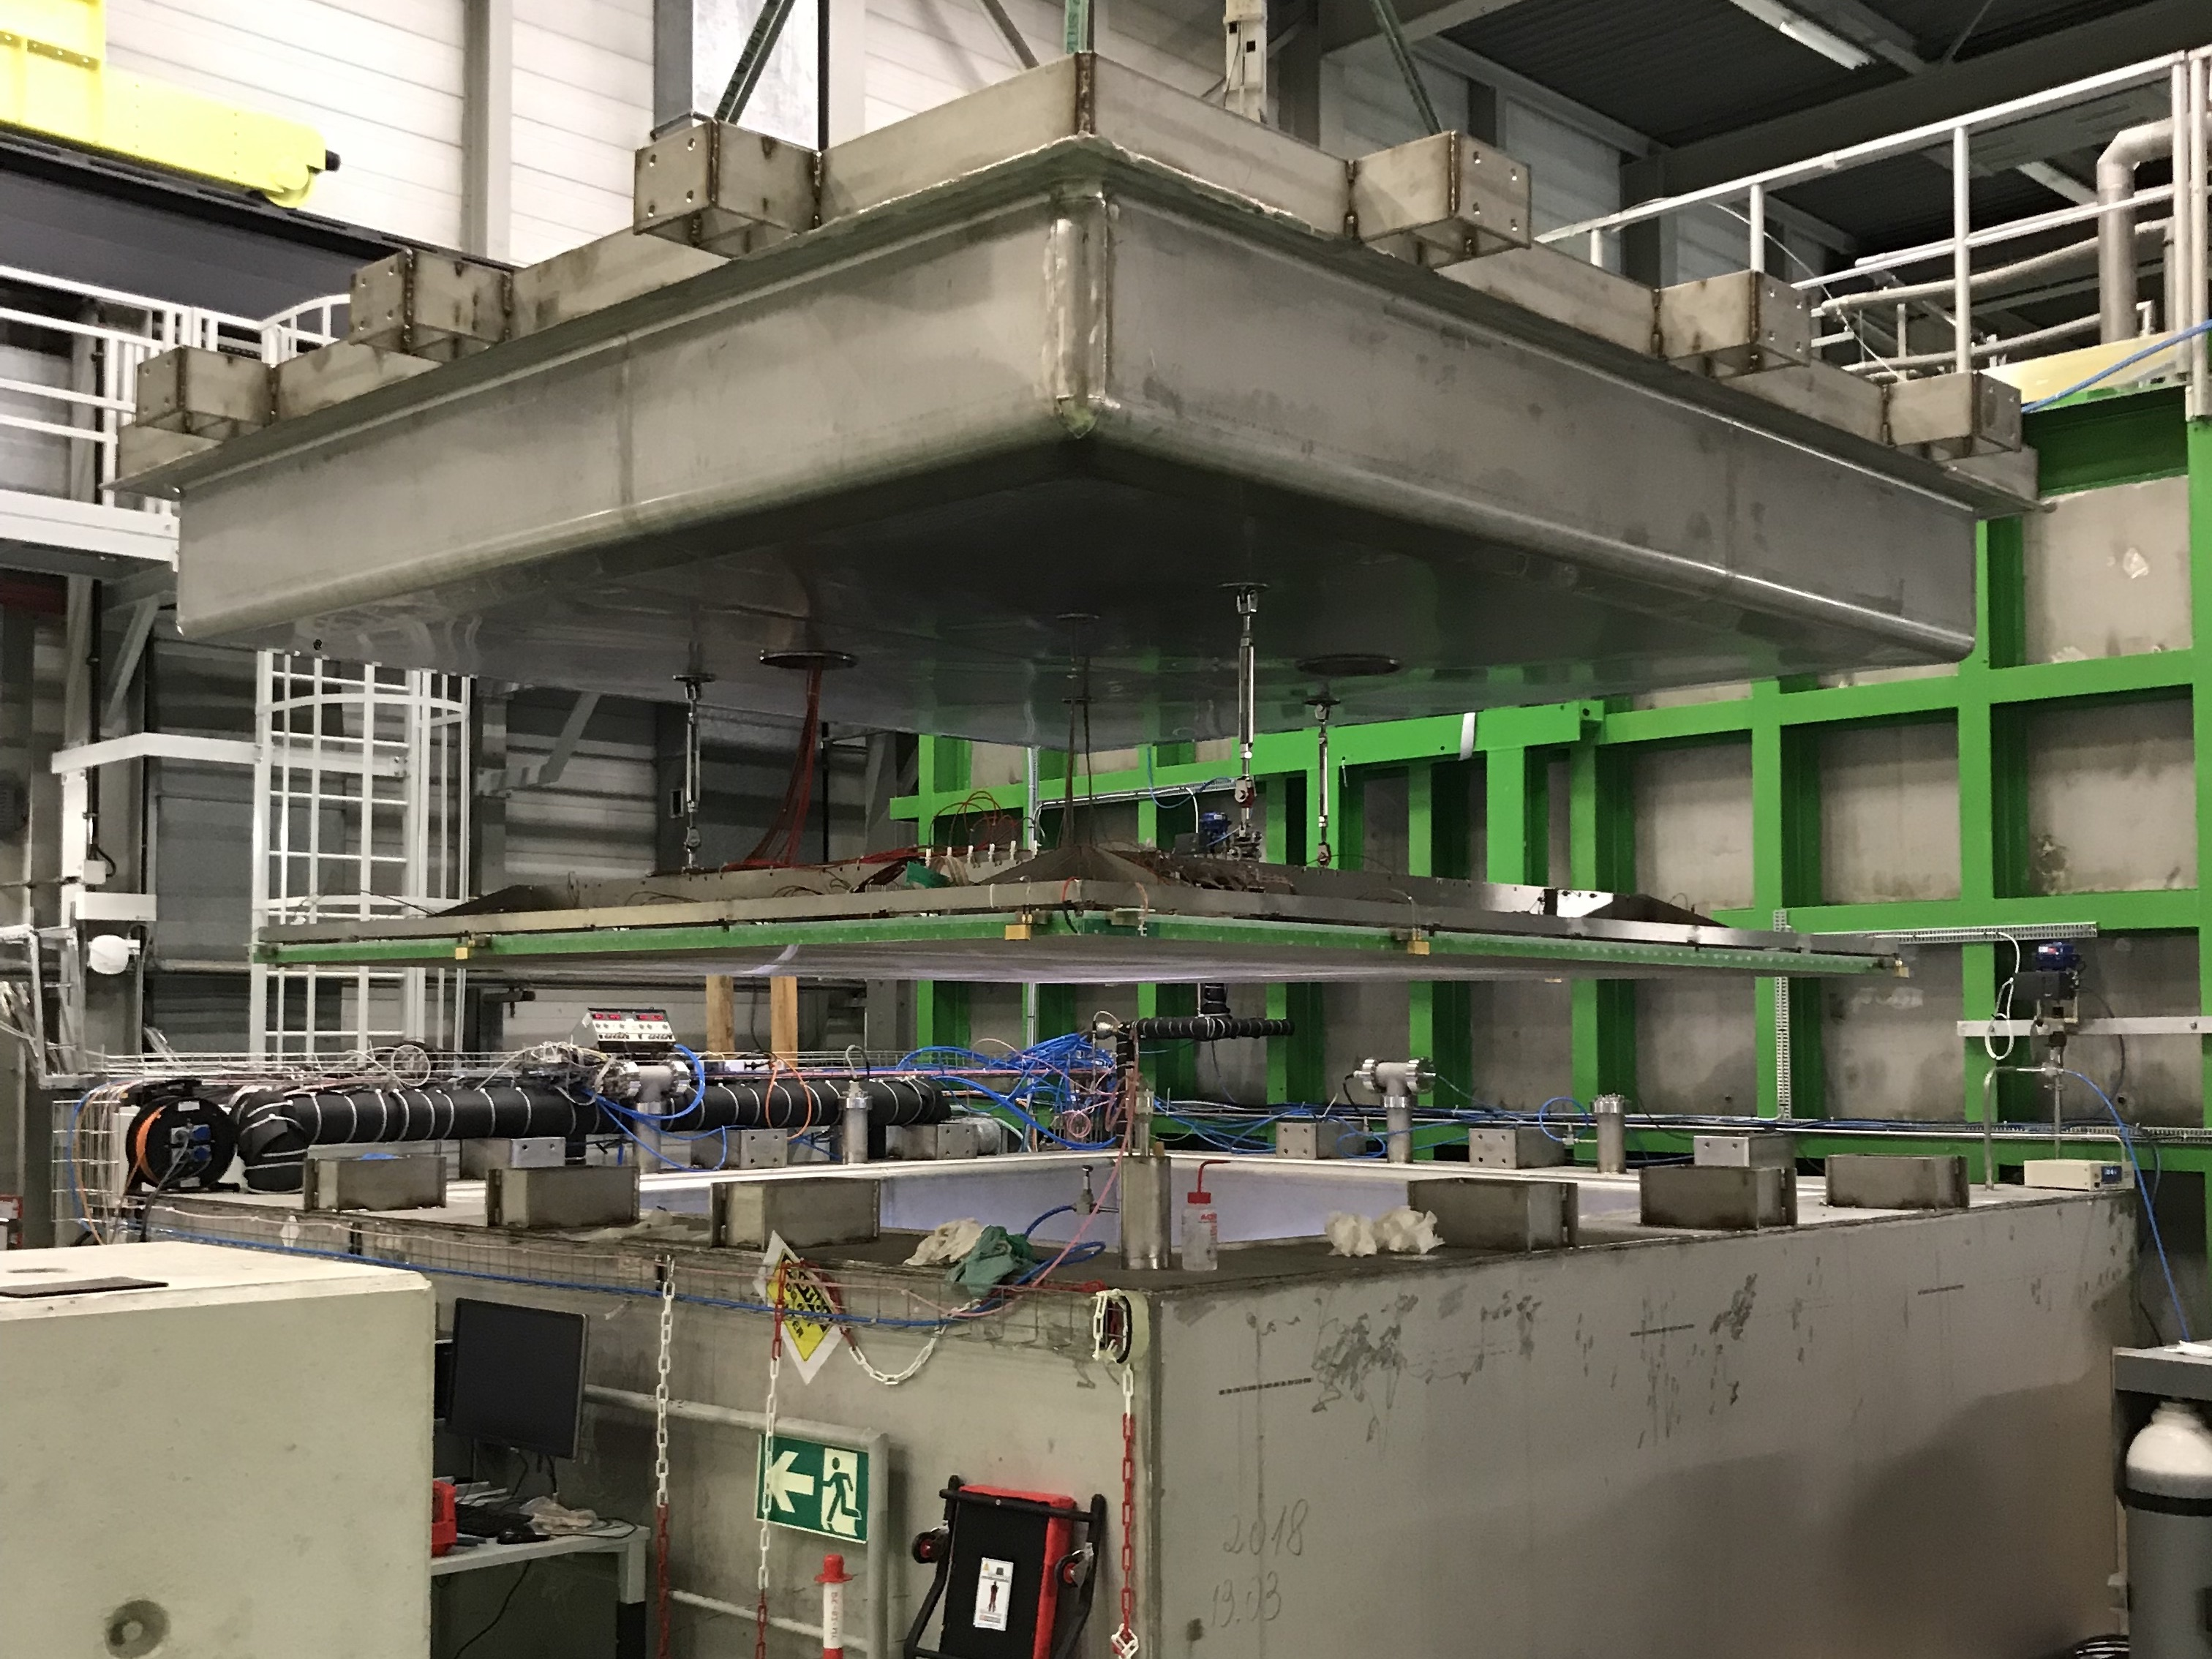
\includegraphics[width=1.\textwidth]{NP02-cold-box.jpg}
\end{dunefigure}

During the tests, the contamination of nitrogen and oxygen was always well below 100~ppm and the measurement was limited by the sensitivity of the instrument.
The level was monitored with a coaxial capacitive level meter and it was also monitored by means of eight capacitive level meter installed around the \dword{crp} with a precision of 250~$\mu$m.
The level was automatically and constantly adjusted to the nominal value refiling the cold box with new liquid argon.
The liquid argon evaporation resulted in a level decrease of about 0.7~mm/h\footnote{The evaporation rate is a simple method to evaluate the heat input due to the cold box only which results in less than 700~W. In the case of the \dword{pddp} cold box, the argon was let evaporate and replaced with new argon to maintain the level.}.
A simplified version of the \dword{pddp} final suspension system allows to adjust the position of the CRP with respect to the liquid argon level using three manual winches changing the height of the CRP at the level of the anchoring points by step of 0.4~mm.
To complete the cold box instrumentation, three cryogenic cameras were used to control the \dword{crp} from below and above.
One camera was positioned to give a side view of the \dword{crp} with a field of view of the order of 40~cm.
In figure~\ref{fig:NP02-ColdBoxCamera} one can appreciate the flatness of the liquid argon level, which is much better than 2~mm even when the regulation of the liquid argon level is functioning.
\begin{dunefigure}[Image from inside the \dword{pddp} cold box]{fig:NP02-ColdBoxCamera}
{Photo from the inside of the \dword{pddp} cold box at \dword{cern} during a \dword{crp} test.}
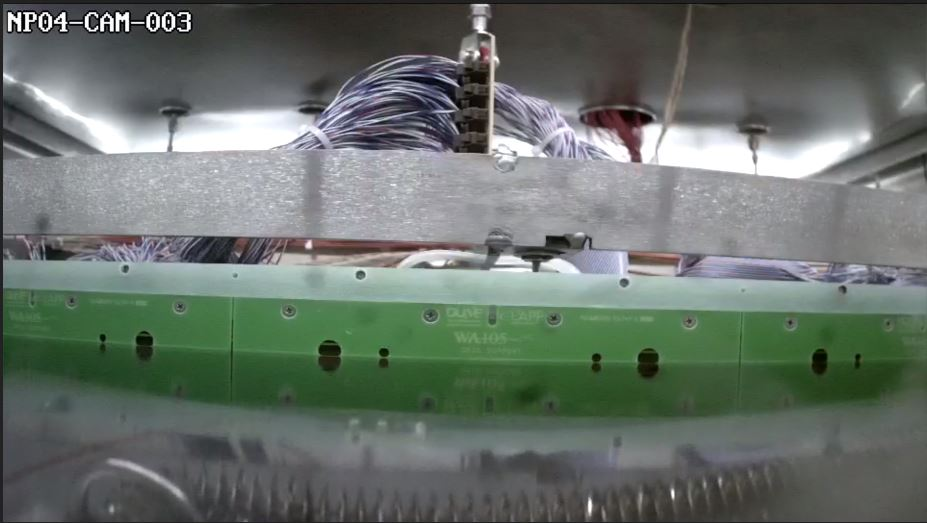
\includegraphics[width=1.\textwidth]{NP02-ColdBoxCamera.jpg}
\end{dunefigure}

\subsection{Alternative position of the cold boxes}
IN CASE THE DP IS NOT THE SECOND DETECTOR THERE IS NO SPACE IN FRONT OF THE CRYOSTAT AND ADIFFERENT SPACE MUST BE ARRANGED FOR THE CLEAN ROOM AND THE COLD BOXES.
\begin{dunefigure}[]{fig:}
{.}
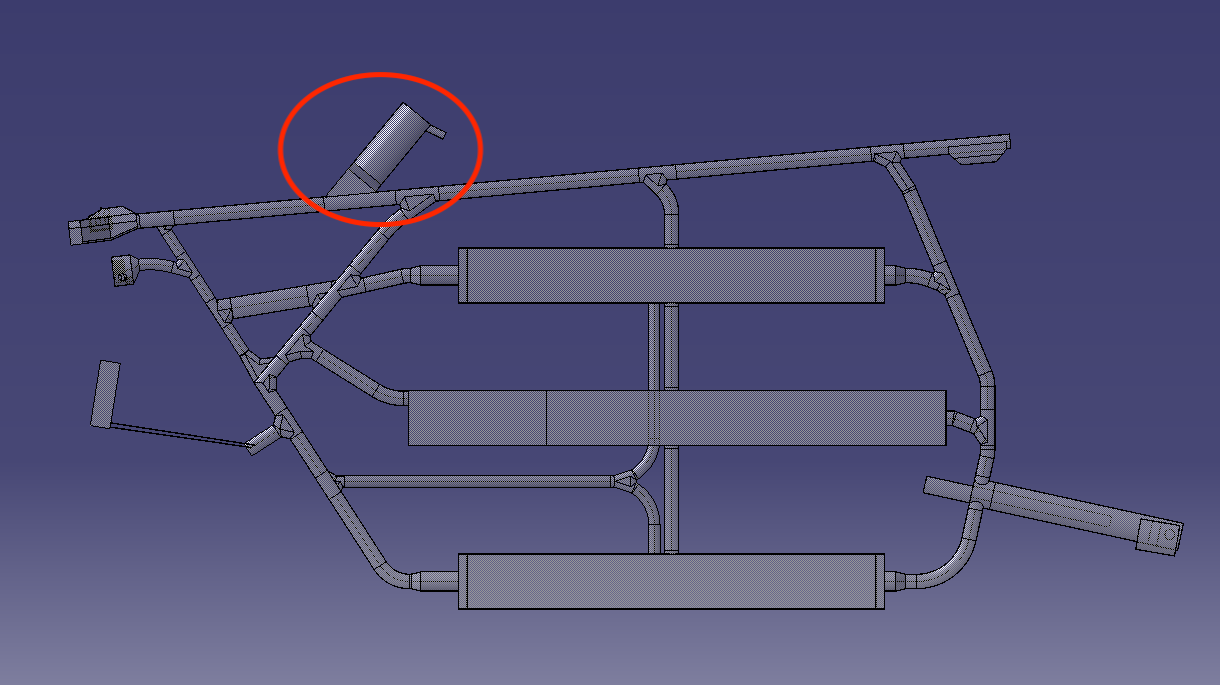
\includegraphics[width=1.\textwidth]{image001.png}
\end{dunefigure}
